 % mnras_template.tex 
%
% LaTeX template for creating an MNRAS paper
%
% v3.0 released 14 May 2015
% (version numbers match those of mnras.cls)
%
% Copyright (C) Royal Astronomical Society 2015
% Authors:
% Keith T. Smith (Royal Astronomical Society)
%
% v3.0 May 2015
%    Renamed to match the new package name
%    Version number matches mnras.cls
%    A few minor tweaks to wording
% v1.0 September 2013
%    Beta testing only - never publicly released
%    First version: a simple (ish) template for creating an MNRAS paper

%%%%%%%%%%%%%%%%%%%%%%%%%%%%%%%%%%%%%%%%%%%%%%%%%%
% Basic setup. Most papers should leave these options alone.
\documentclass[useAMS,usenatbib]{mnras}

% MNRAS is set in Times font. If you don't have this installed (most LaTeX
% installations will be fine) or prefer the old Computer Modern fonts, comment
% out the following line
\usepackage{newtxmath}
%\usepackage{newtxtext}
\RequirePackage{amsfonts}
% Depending on your LaTeX fonts installation, you might get better results with one of these:
%\usepackage{mathptmx}
%\usepackage{txfonts}
\usepackage{hyperref}
%\hypersetup{draft}
\usepackage{natbib}
\usepackage{xcolor}
\newcommand\todo[1]{\textcolor{red}{#1}}

% Use vector fonts, so it zooms properly in on-screen viewing software
% Don't change these lines unless you know what you are doing
\usepackage[T1]{fontenc}
\usepackage{ae,aecompl}


%%%%% AUTHORS - PLACE YOUR OWN PACKAGES HERE %%%%%

% Only include extra packages if you really need them. Common packages are:
\usepackage{graphicx}	% Including figure files
\usepackage{amsmath}	% Advanced maths commands
\usepackage{amssymb}	% Extra maths symbols
\usepackage{bm}      	%for bold italic symbol, vector
\usepackage{gensymb}  	%for degree
%\usepackage{auto-pst-pdf}
\usepackage{makecell}
\usepackage{multirow}
\usepackage{url}

%%%%%%%%%%%%%%%%%%%%%%%%%%%%%%%%%%%%%%%%%%%%%%%%%%

%%%%% AUTHORS - PLACE YOUR OWN COMMANDS HERE %%%%%
\newcommand\rxj{RXJ\,1131$-$1231}
\newcommand\he{HE\,0435$-$1223}
\newcommand\pg{PG\,1115$+$080}
\newcommand\bb{B\,1608$+$656}
\newcommand{\sref}[1]{Section~\ref{#1}}
\newcommand{\fref}[1]{Figure~\ref{#1}}
\newcommand{\tref}[1]{Table~\ref{#1}}
\newcommand{\eref}[1]{Equation~(\ref{#1})}
\def\mathbi#1{\textbf{\em #1}}
\def\hst{\textit{HST}}
\def\planck{\textit{planck}}
\def\WMAP{\textit{WMAP}}
\def\zl{z_{\ell}}
\def\zs{z_{s}}
\def\nomicro{$\cdots$}
\def\nodata{$\cdots$}
%\def\Ddt{d_{\Delta t}}
\def\kms {\rm km\,s^{-1}}
\def\kmsmpc{\rm km\,s^{-1}\,Mpc^{-1}}
\newcommand{\Ddt}{D_{\Delta t}}

% Please keep new commands to a minimum, and use \newcommand not \def to avoid
% overwriting existing commands. Example:
%\newcommand{\pcm}{\,cm$^{-2}$}	% per cm-squared

%%%%%%%%%%%%%%%%%%%%%%%%%%%%%%%%%%%%%%%%%%%%%%%%%%

%%%%%%%%%%%%%%%%%%% TITLE PAGE %%%%%%%%%%%%%%%%%%%

% Title of the paper, and the short title which is used in the headers.
% Keep the title short and informative.
\title[$H_{0}~from~three~lenses~with~AO~imaging$]{SHARP. $H_{0}$ from adaptive optics imaging of three gravitational lens systems}
%\uppercase\expandafter{\romannumeral 5
%
% The list of authors, and the short list which is used in the headers.
% If you need two or more lines of authors, add an extra line using \newauthor
\author[G.~ C.-F.~Chen et al.]{
G.~C.-F.~Chen,$^{1}$ \thanks{E-mail: chfchen@ucdavis.edu}
C.~D.~Fassnacht,$^{1}$
%S.~H.~Suyu,$^{2,3}$
%C.~E.~Rusu,$^{1}$
%A. Halkola,
\newauthor{
%M.~W.~Auger,$^{6}$
%L.~V.~E.~Koopmans,$^{7}$
%D.~J.~Lagattuta,$^{8}$
%J.~P.~McKean,$^{7,9}$
%S.~Vegetti,$^{2}$
}
\newauthor{
%V.~Bonvin,
%J.~Chan,
%F. Courbin,
%??
}
\\
% List of institutions
$^{1}$Department of Physics, University of California, Davis, CA 95616, USA\\
%$^{2}$Max $\planck$ Institute for Astrophysics, Karl-Schwarzschild-Strasse 1, D-85740 Garching, Germany\\
%$^{3}$Institute of Astronomy and Astrophysics, Academia Sinica, P.O.~Box 23-141, Taipei 10617, Taiwan\\
%$^{4}$Institute of Astrophysics, National Taiwan University, Taipei 10617, Taiwan\\
%$^{5}$Center for Theoretical Sciences, National Taiwan University, Taipei 10617, Taiwan\\
%$^{6}$Institute of Astronomy, University of Cambridge, Madingley Rd, Cambridge, CB3 0HA, UK\\
%$^{7}$Kapteyn Astronomical Institute, University of Groningen, P.O.Box 800, 9700 AV Groningen, The Netherlands\\
%$^{8}$CRAL, Observatoire de Lyon, Universit Lyon 1, 9 Avenue Ch. Andr, F-69561 Saint Genis Laval Cedex, France\\
%$^{9}$Netherlands Institute for Radio Astronomy (ASTRON), P.O. Box 2, 7990 AA Dwingeloo, The Netherlands \\
}

% These dates will be filled out by the publisher
\date{Accepted XXX. Received YYY; in original form ZZZ}

% Enter the current year, for the copyright statements etc.
\pubyear{2015}

% Don't change these lines 
\begin{document}
\label{firstpage}
\pagerange{\pageref{firstpage}--\pageref{lastpage}}
\maketitle

% Abstract of the paper
\begin{abstract}
Time-delay strong lensing provides an independent way to measure the Hubble constant ($H_{0}$). 
We present the blind analysis of both \pg~and \he~as well as the analysis of \rxj. For each lens, we combine the adaptive optics (AO) imaging from Keck telescope, the Hubble space telescope (\hst) imaging, the time delays, the velocity dispersions, and the line of sight to infer the $H_{0}$. After unblinding, \he~implies the Hubble constant $H_{0}=xx$; \pg~implies $H_{0}=xx$. The joint results of three lenses is $H_{0}=xxx$ assuming a flat-$\Lambda$ cold dark matter cosmology with uniform prior on $\Omega_{\textrm{M}}$ in [0.05, 0.5]. This work is under the collaboration of SHARP team and H0LiCOW team. 
\end{abstract}

% Select between one and six entries from the list of approved keywords.
% Don't make up new ones.
\begin{keywords}
gravitational lensing: strong -- instrumentation: adaptive optics -- distance scale.
\end{keywords}

%%%%%%%%%%%%%%%%%%%%%%%%%%%%%%%%%%%%%%%%%%%%%%%%%%

%%%%%%%%%%%%%%%%% BODY OF PAPER %%%%%%%%%%%%%%%%%%

\section{Introduction}
%The standard flat $\Lambda$-CDM model has became a concordance cosmological model \citep{$\planck$16a} after the discovery of the acceleration of universe \citep{PerlmutterEtal99,RiessEtal98}. 
%consolidate the need for the extra energy density, which fills out the budgetary shortfall of the energy density due to the flatness of the universe. After that, the standard $\Lambda$-CDM model became a concordance cosmological model, which assumes the spatial flatness and the matter content dominated by cold dark matter but with dark energy which causes the accelerated expansion. 
%This simple model with a few strong assumptions unexpectedly
%which describes the universe with a minimal set of six parameters, 
%provides an excellent fit to the various observable effects, including 


The temperature anisotropy of the cosmic microwave background (CMB) and density correlation of Baryon Acoustic Oscillations (BAO) obtained with the Wilkinson Microwave Anisotropy Probe, $\planck$ satellite, and the BAO surveys provide strong supports to the standard flat $\Lambda$-CDM model \citep[e.g.,][]{KomatsuEtal11,HinshawEtal13,planck18parameter}. With a few strong assumptions, these data give unprecedented sub-percent precision on the parameters of the standard cosmological model
 \citep[e.g.,][]{AndersonEtal14,KazinEtal14,RossEtal15}.

Intriguingly, the distance measurements from Type-Ia supernova (SN) calibrated by local distance ladder are marginally smaller than the prediction from the flat $\Lambda$-CDM model given CMB data \citep[see Fig. 4 in][]{CuestaEtal15}. 
It leads to the current $\sim 3\sigma$ tension of a higher value of $H_{0}$ ($=73.48\pm1.66~\kmsmpc$) under the assumption of the standard cosmological model \citep{RiessEtal18c}. 
On the other hand, SN data can also be calibrated by the inverse distance ladder to yield a model-dependent $H_{0}$.
With the assumption of the standard pre-recombination physics and the number of effective neutrino species, $N_{\textrm{eff}}$, combining BAO and SN with the CMB-calibrated physical scale of the sound horizon, $r_{s}$, gives $H_{0} =67.3\pm1.1~\kmsmpc$ \citep{AuborugEtal15}, and recently with the additional SN data from Dark Energy Survey, \citet{MacaulayEtal18} obtain $H_{0} =67.77\pm1.30~\kmsmpc$. Both results are in an excellent agreement with the $\planck$ value ($H_{0} = 67.27\pm0.6~\kmsmpc$) under the assumption of flat $\Lambda$-CDM model \citep{planck18parameter}. Furthermore, even without using CMB anisotropy, combining BAO data with light element abundance, which is used to determine the baryon-to-photon ratio and thus $r_{s}$ (fixed $N_{\textrm{eff}}=3.046$), produces $\planck$-like $H_{0}$ values \citep{AddisonEtal18}. This indicates that systematic errors, especially in the $\planck$ data analysis, most likely are not the main driver of the $H_{0}$ discrepancies. 
 Likewise, the distance ladder analyses also have passed a range of systematic checks including replacing rungs of the ladder with alternative data, revising for estimated local motion, and considering a range of modeling variants
 \citep[e.g.,][]{Efstathiou14,CardonaEtal17,ZhangEtal17,FollinKonx18,FeeneyEtal18,DhawanEtal18}. 
 Additionally, a local void centered on our galaxy, which could produces positive peculiar velocities for the nearby galaxies and hence bias local $H_{0}$ measurements \citep{KeenanEtal13,FleuryEtal17,ShanksEtal19}, was ruled out with $5\sigma$ by using the currently largest SN samples \citep{KenworthyEtal19}.

There are several attempts to address this $\sim 3\sigma$ tension by the extension of the standard cosmological model. 
Since the CMB data give an astonishingly precise measurement on $\theta_{s}$ \citep[$\sim 0.05\%$;][]{planck18parameter}, the ratio of $r_{s}$ to the angular diameter distance to the last-scattering surface, modifying $r_{s}$ leads to changing the overall inferred distance. 
%Thus, the first attempt is to change the early-time physics, which can affect the sound horizon. 
For example, if one increases $N_{\textrm{eff}}$, the expansion rate becomes more rapid in the early universe and also the radiation-matter equality shifts to earlier times, which causes a smaller $r_{s}$ and thus brings both CMB- and BAO-based $H_{0}$ values close to the SN measurement \citep[e.g.,][]{HouEtal14,HeavensEtal14,WymanEtal14,CuestaEtal15}.
%To remain the statistical property of the CMB data, the overall distance decreases and agree with the direct distance measurements from SN. 
However, to keep $\theta_{s}$ fixed, increasing $N_{\textrm{eff}}$ leads to increasing $H_{0}$, and since the observed diffusion length is proportional to the square root of the Hubble parameter, the amount of damping on the high-$\ell$ CMB power spectrum is enhanced. %and makes it sensitive to the angular scale of the diffusion length, $\theta_{d}$
\citep[e.g.,][]{Silk68,HouEtal13,planck16a}. Therefore, $\planck$ data alone still favor $N_{\textrm{eff}}= 2.97\pm0.2$ ($H_{0}=66.6\pm1.6~\kmsmpc$) under the assumption of the $\Lambda$CDM model + free $N_{\textrm{eff}}$ \citep{AlamEtal17}. On the other hand, \citet{KreischEtal19} just pointed out that the self-interaction neutrinos could compensate the suppressing from increasing $N_{\textrm{eff}}$, which can accommodate a high $H_{0}$ value without degrading the fit to the damping tail, but Bayes statistics disfavor the model due to the narrow window of suitable interaction strength. In addition, early dark energy could also change $r_{s}$ but the allowable shift of $H_{0}$ is very limited given the CMB data \citep{PoulinEtal18}. %The last two scenarios can be examined by future observation \citep[e.g.,][]{CMB-S4}.

%In addition, \citet{ChiangSENVar18} proposed a modification to the timing and width of the recombination process which can affect the size of sound horizon, but this modification by adding more parameters mostly broaden the uncertainties rather than shift the $H_{0}$ value when they consider the full $\planck$ data.

Conversely, if we do not alter the pre-recombination physics but modify the expansion history, the normalization (i.e., $H_{0}$) needs to be changed accordingly in order to maintain the same distance to the last scattering surface \citep{RiessEtal16,Freedman17}.
%Since $H_{0}$ is the 
%Based on assumptions of the early time physics and the late time expansion of the universe, the CMB data obtained with $\planck$ satellite can be used to infer the Hubble constant ($H_{0}$), an important absolute distance scale of the universe, which sets the age, size, and critical density of the universe. 
%Intriguingly, the recent inferred value of $H_{0}=67.8\pm0.9\kms$\citep{AdeEtal15}, based on $\planck$ data of CMB by assuming the flat $\Lambda$CDM model, is marginally lower than the direct measurements based on distance ladder of 73.24$\pm$1.74 \citep{RiessEtal16} and of $74.3\pm2.1$ \citep{FreedmanEtal12}. Besides, the recent Dark Energy Survey year 1 (DESY1) results also show that, the preference for the smaller matter density, together with CMB data, break the degeneracy and lead to a shift in the direction of local measurements \citep[see Fig. 12 in][]{DEScollaboration17}.
%On the other hand, $\planck$ results agree with the results from the mega-maser measurements \citep[e.g.,][]{ReidEtal13,KuoEtal15,GaoEtal16}.
%Although CMB provides most precise measurements of $H_{0}$, if one relaxes the assumptions such as the flatness of curvature, the effective number of neutrino species, and the dark energy equation of state, $w=-1$, a strong degeneracy in the parameters space appear. \citep{BernalEtal16, RiessEtal16}
For example, if one decreases the dark energy equation of state, this decreases the contribution of the dark energy density to the shape of the expansion rate, and thus increases the overall distance to the last scattering surface \citep[e.g.,][]{Linder04}; if one increases the curvature energy density, the negative curvature will also increase the predicted distance \citep[e.g.,][]{EfstathiouEtal03}. 
Above solutions require a higher value of $H_{0}$ to fit the $\theta_{s}$ and thus strong degeneracies in the parameter space, especially with $H_{0}$, appear \citep{planck18parameter}. However, if one further includes BAO, SN, or the differential evolution of cosmic chronometers, which act as a hinge at low redshift, zero curvature and constant dark energy equation of state are still preferred \citep[e.g.,][]{MorescoEtal16,AlamEtal17} under the assumption of the common parametric form of dark energy \citep{Linder03}.

%Therefore, direct measurement of the value of $H_{0}$ to 1\% uncertainty is highly needed to empirically investigate the assumptions \citep{SuyuEtal12b}.
% or understand the possible systematic uncertainties 
%Furthermore, \citet{WeinbergEtal13} also points out that for the stage IV Dark energy program, assuming a $w_{0}- w_{a}$ model (non-constant dark energy equation of state) for dark energy, the Figure of Merit will improve by 40\% if we can measure $H_{0}$ to 1\%.

%Furthermore, there are also cosmological models, beyond standard extension of $\Lambda$-CDM, which were proposed to explain the higher $H_{0}$ values. \citet{Romano16} Romano addressed this question by saying that it is due to the fact that we live in an under-dense region. If we account for the void, the tension can be resolved.
%\citet{RaczEtal17} propose that the nonlinear deviations from a homogeneous FLRW universe (voids and walls) are too great to to account for with perturbation theory. Their numerical simulation models a matter-only CDM universe with a series of what they call “mini-universes,” each with their own local $\Omega_m$ and expansion. They claim that dark energy can be entirely accounted for in this model, as well as the discrepancy between supernova and CMB $H_0$ measurements. 
In addition to the standard extension, recent studies \citep[e.g.,][Jee et al. submitted]{BernalEtal16,LemosEtal18,JoudakiEtal18,AylorEtal18} have tried to directly reconstruct $H(z)$ in order to investigate the $H_{0}$ tension due especially to the poor understanding of the evolution of dark energy density. From an empirical point of view, the current dataset of SN together with BAO only support $w(z)=-1$ within 
%$z=0.03\sim z=3$ 
the redshift range where data is available \citep{CuestaEtal16}. A very recent and dramatic decrease in $w$ or the presence of strong dark energy at $3 <z < 1000$ may escape detection and still generate a high value of $H_{0}$ \citep{RiessEtal16}.
Nevertheless, it is also important to note that some $H_{0}$ tension remains even if we do not consider the distance ladder constraints. 
For example, the high-$\ell$ CMB power spectrum prefers an even lower $H_{0}$ value than that from the low-$\ell$ CMB power spectrum \citep{AddisonEtal16,planck18parameter}, although \citet{Planck16c} claims that this is not statistically significant. Given the various mild tensions across different datasets, any convincing resolution, either due to unknown systematics or new physics, needs to simultaneously resolve multiple disagreements. 
Therefore, comparing the distance measurements among independent and solid methodologies is probably the only way to cross-exam the $H_{0}$ tension and shed light on the true answer.

%Note that SN can only yield the shape of the expansion rate rather than $H_{0}$ without calibration from a local distance ladder or from the model-dependent inverse distance ladder \citep{CuestaEtal16}. Due to the fact that the tension mainly comes from the calibrated SN by the local distance ladder, the unknown systematics in the local distance ladder %or the local void 
%can be also a possible explanation. %However, the latter requires a extremely fine tune and is disfavored by the Hubble diagram of SNe we 
%Thus, using multiple independent methodologies to measure the value of $H_{0}$ is crucial to exam the systematics.

In contrast to SN, time-delay strong lensing (TDSL) is not only a completely independent technique, but also a one-step measurement of combined cosmological distances without the need of calibration. In addition, when compared with Type-Ia SN or BAO, TDSL is a complementary and cost-effective alternative \citep{SuyuEtal13,TewesEtal13a}.
In a time-delay lens, the combined cosmological distance we can measure is called time-delay distance \citep[$\Ddt$; see the review by][]{TreuMarshall16, SuyuEtal18} and, furthermore, we can obtain the angular diameter distance to the lens ($D_{\ell}$) by measuring the velocity dispersion of the lensing galaxy \citep{JeeEtal15,JeeEtal16,BirrerEtal18}. 
%More recently, \citet{GrilloEtal16,GrilloEtal18} show that it is possible to measure precisely of $H_{0}$ by the spectroscopic multiply-lensed sources and the time delays between the multiple images of a variable source in the lens galaxy cluster.
First proposed by \citet{Refsdal64}, the measurement involves modeling the mass along the line of sight and monitoring the time delays between multiple images. 
More specifically, 
\begin{equation}
\label{eq:TDeq}
\Delta t=(\Ddt/c)\Delta\phi,
\end{equation}
where $\Delta t$ is time delays between imagings, $\Delta\phi$ is the difference of the Fermat potential between images, and c is the speed of light. 
The advantage of this method is that $\Ddt$ is primarily sensitive to $H_{0}$ and insensitive to the neutrino physics and spatial curvature, but still sensitive to the property of dark energy \citep{BonvinEtal17,BirrerEtal18}.

%However BAO, together with the CMB, can be served as an "inverse distance ladder" to calibrate the absolute magnitude of SN by assuming the absolute magnitude of the supernova does not evolve with time, which is insensitive to the dark energy properties and spatial curvature \citep{AuborugEtal15}. 
%Even so, using the inverse distance ladder to calibrate the SN depends on the sound horizon which is still model-dependent \citep{CuestaEtal15}.

The most recent precise $H_{0}$ measurement from strong lensing was done by the H0LiCOW group\footnote{\url{www.h0licow.org}} %, with the aim of measuring the Hubble constant with better than $3.5\%$ precision and accuracy
\citep[H0 Lenses in COSMOGRAIL’s Wellspring,][]{suyuEtal17}. With the improvement on controlling the possible microlensing time-delay effect \citep{TieKochanek18,GChenEtal18a} and the usage of different modeling techniques \citep{BirrerEtal15,BirrerAmara18}, \citet{BirrerEtal18} obtain $H_{0}=68.8\substack{+5.4\\-5.1}~\kmsmpc$ with the doubly imaged quasar SDSS 1206+4332 and $H_{0}=72.5\substack{+2.1\\-2.3}~\kmsmpc$ by combining \citet{FassnachtEtal02} and the previous H0LiCOW work \citep{SuyuEtal09,SuyuEtal10,SuyuEtal13,SuyuEtal14,SluseEtal17,RusuEtal17,WongEtal17,BonvinEtal17}. This result agrees with \citet{RiessEtal18c}.

%H0LiCOW group carefully study the environment of the \he~by using the spectroscopic follow-up of the strong lens field and using the flexion shift to identify the important group/galaxy along the line of sight \citep{SluseEtal17}.
%\citet{RusuEtal17} estimated the mass contribution from the environment by ray-tracing the numerical simulations in combination with multi-band data, which is later confirmed by weak lensing analysis \citep{TihhonovaEtal17}. 
%Combining the environment study with the lens modeling  of \he~\citep{WongEtal17} and the previous studies of \rxj~and \bb~\citep{SuyuEtal09,SuyuEtal10,SuyuEtal13,SuyuEtal14}, \citet{BonvinEtal17} gives the $H_{0}=71.9^{+2.4}_{-3.0}$ in the flat $\Lambda$-CDM model, which agrees with \citep{RiessEtal16}. 

To achieve the goal of 1\% $H_{0}$ measurement with TDSL, the state-of-the-art lens-finding techniques applied to current large sky surveys \citep[e.g.][]{JosephEtal14,AvestruzEtal17,Agnello17,PetrilloEtal17,OstrovskiEtal17,LanusseEtal18}, have already shown promising results. Many new lenses have been discovered \citep[e.g.,][]{LinEtal17,AgnelloEtal17, SchechterEtal17,OstrovskiEtal18,WilliamEtal18,RusuEtal18,LemonEtal19,DelchambreEtal19} and thousands of lensed quasars are expected to be found with the Large Synoptic Survey Telescope \citep{OguriMarshall10}.
Hence, a 1\% $H_{0}$ measurement from time-delay cosmography is a realistic expectation in the near future \citep[e.g.,][Jee et al. 2018 submitted]{JeeEtal15,JeeEtal16,deGrijsEtal17,SuyuEtal18,ShajibEtal18} if we can control the systematic effects to a sub-percent level \citep[][]{DoblerEtal13,LiaoEtal15,DingEtal18}.

Since high-resolution imaging and a well-known Point Spread Function (PSF) are essential for modeling the lens potential, HST imaging data serve as good datasets widely used for modeling strong lenses \citep[e.g.,][]{SuyuEtal09,SuyuEtal10,BirrerEtal15,WongEtal17,BirrerEtal16,BirrerEtal18}. However, as HST is limited by its aperture size (and thus its resolution), lens modeling uncertainties can be the dominant term in terms of measuring the value of $H_{0}$ \citep[e.g.,][]{SuyuEtal14}.
Adaptive optics (AO) imaging obtained from ground-based telescopes can not only further help constrain the lens mass distribution, but also serve as an alternative for modeling the lens mass distribution \citep{GChenEtal16}.
%it cannot provide as sharp imaging as larger telescopes. 
%can't last forever and the resolution is limited by its aperture size, especially considering the hundreds of new lenses to be discovered in the near future  \citep{OguriMarshall10,AgnelloEtal15,ChanEtal15,MarshallEtal15,MoreEtal15,Agnello17}, 
%Thus, adaptive optics (AO) imaging  is 

%The idea of AO system is that since turbulence in the earth atmosphere will distort the light of celestial objects making astronomical image blurry and ground-based telescope cannot avoid the atmosphere like the space telescope can, the adaptive optics facility launches the lasers to creates artificial stars in the upper atmosphere and an adaptive optics module uses this stars to map the turbulence in the atmosphere. 
%This deformable mirror can rapidly changes its shape to correct the wavefront it receives from the celestial objects compensating for the atmospheric disturbance \citep[e.g.,][]{RoussetEtal90,Beckers93,Watson97,Brase98}. 
%The advantages of AO imaging are the angular resolution obtained with telescopes that are larger than \textsl{HST} can be higher than that of \textsl{HST} since a perfect AO system would lead to a diffraction-limited PSF and the ground-based telescopes are more accessible. 
However, the challenge of using AO data is the unstable PSF, which sets a main obstacle for using AO imaging. %In order to overcome this challenge, varies methods for different science goals have been developed to model the PSF. \citep{Lagattuta10,RusuEtal16,AgnelloEtal15_2}
%\citet{Lagattuta10} uses three Gaussian components to subtract the the AGN light, which is sufficient for studying lens galaxy and its substructure. \citet{RusuEtal16} use either an analytic or a hybrid PSF to model the AGN light, which is sufficient for studying the host galaxies of the lensed AGNs. \citet{AgnelloEtal15_2} iteratively reconstructed the PSF from the two lensed AGNs, which is sufficient for forecasting the cosmological inference. 
\citet{GChenEtal16} show that with a new iterative PSF-reconstruction method, the reconstructed PSF allows one to model the AO imaging down to the noise level, as well as providing tighter constraint on the lens model. 
In this paper, we apply the PSF-reconstruction method on the three lens systems, \rxj, \he, \pg, which have not only high-resolution AO imaging and HST imaging, but also measured time delays, velocity dispersion, and studies of environment, to infer their time-delay distances. 
The Keck AO imaging data are part of SHARP\footnote{Strong-lensing High Angular Resolution Programme (Fassnacht et al. in preparation)}, which aims to study dark matter substructures using high-resolution AO imaging \citep[e.g.,][]{Lagattuta10,Lagattuta12,Vegetti12,Hsueh16,HsuehEtal17_Illustris,HsuehEtal17_edgeon}.
The time delay measurements are provided by the COSMOGRAIL\footnote{COSmological MOnitoring of GRAvItational Lenses} group \citep[e.g.,][]{CourbinEtal05,VuissozEtal07,VuissozEtal08,CourbinEtal11,TewesEtal13b,TewesEtal13a,RathnaEtal13,BonvinEtal17}, which aims to provide the highest-precision measurements of time delays. The lens environment of \rxj and \he studies are provided by H0LiCOW team \citep{SuyuEtal14,SluseEtal17,RusuEtal17}.

The outline of the paper is as follows. In Section \ref{sec:basic}, we briefly recap the basics of cosmography with time-delay lenses and the statistical tool we use for cosmological inference. We describe the observation of \rxj, \he, \pg, with the AO imaging system at the Keck Observatory in section \ref{sec:data}. In section \ref{sec:modeling_tool}, we describe the models we use to analyze the data, and the properties of the reconstructed PSF for each system. We summarize in Section \ref{sec:conclusion}.



\section{Basic theory}
\label{sec:basic}
In this section, we briefly introduce the relation between cosmology and gravitational lensing in \sref{sec:TDcosmo} and the joint inference of all information in \sref{sec:Jointinfer}.

\subsection{Time-delay cosmography}
\label{sec:TDcosmo} % used for referring to this section from elsewhere
When a compactly light-variable background source, such as active galactic nuclei (AGN) or SN, sitting inside its host galaxy, is strongly lensed by a foreground object, the distorted host galaxy shape, combined with the time delay between the multiple images allows one to precisely determine a particular size of the system. One can express the excess time delays as
%the light ray would be bended by the gravitational field. The time delays  between mutliple images allow one to overall scale of the 
%The photon experience two components of time delay: (1) the geometry delay,  which is caused by different trajectory, and (2) the Shapiro delay, which is caused by the gravitational potential. 
%We can express the time delay as 
\begin{equation}
\label{eq:theory}
t=(1-\lambda)\frac{\Ddt}{c}\left[\frac{1}{2}
\left(\boldsymbol{\theta}-\boldsymbol{\beta}\right)^{2}-\psi\left(\boldsymbol{\theta}\right)\right],
\end{equation}
where $\bm{\theta}$, $\bm{\beta}$, and
$\psi\left(\bm{\theta}\right)$ are the image coordinates, the source
coordinates, and the lens potential, respectively \citep{Shapiro64, Refsdal64}.
The time delay distance, which links to the cosmological parameters, % inversely proportional to $H_{0}$ 
is defined as
\begin{equation}
\label{eq:TDdistance}
\Ddt\equiv\left(1+
\zl\right)\frac{D_{\ell}D_{s}}{{D_{\ell s}}}\propto H_{0}^{-1},
\end{equation}
where $D_{l}$, $D_{s}$ and $D_{\ell s}$ are the angular diameter distances to the lens, to the source, and between the lens and the source, respectively. 
%In reality, one cannot measure the excess delay because the light travel time without the foreground lens is unobservable, whereas if a background source locates inside the strongly lensed region, where the compact source can form multiple images and the smooth source can form a extended images (a.k.a. arc), the delays between the multiple imagings are observable.
%whereas the true observables is the time delay between the multiple imagings. 
%When the background source locates inside the strong lensing region, where the compact source can form multiple images and the smooth source can form a extended images (arc).%between the multiple imagings.
%one are only able to measure the time delay  
%If the background objects is a compactly light-variable source, such as active galactic nuclei (AGN) or SN, one can monitor the relative time delays \citep[e.g.,][]{FassnachtEtal02,TewesEtal13b,BonvinEtal17,RathnaEtal13,EulaersEtal13,CourbinEtal18} and use the extended images to constrain the source position, as well as the potential \citep[e.g.,][]{WarrenDye03,Koopmans05,VegettiKoopmans09,OguriAlgorithm10,NightingaleDye15,BirrerEtal15}.
%$\bm{\Delta t_{i,j}}$, at 
%$\bm{\theta_{i}}$ and $\bm{\theta_{j}}$ and use extended images (a.k.a. arc) to constrain the source position, $\bm{\beta}$, as well as the potential, $\psi\left(\bm{\theta_{i}}\right), \psi\left(\bm{\theta_{j}}\right)$.
%\begin{equation}
%\Delta t_{i,j}=\frac{\Ddt}{c}\left[\frac{1}{2}
%\left(\boldsymbol{\theta_{i}}-\boldsymbol{\beta}\right)^{2}-\psi\left(\boldsymbol{\theta_{i}}\right)-\frac{1}{2}\left(\boldsymbol{\theta_{j}}-\boldsymbol{\beta}\right)^{2}+-\psi\left(\boldsymbol{\theta_{j}}\right)\right]
%\end{equation}
%-\psi\left(\boldsymbol{\theta_{j}}\right)\right],
Because of the Mass-Sheet Transformation (MST) \citep{FalcoEtal85,SchneiderSluse13,SchneiderSluse14}, the determination of $\Ddt$ is subject to the understanding of a free parameter, $\lambda$ \citep[see also the discussion in][]{BirrerEtal18}. Thus, additional prior/information from simulations, environment data, and the velocity dispersion of the lensing galaxy are required to constrain the degeneracy among the choice of different mass profiles and the degeneracy between the mass profile and the mass sheet contributed by the environment \citep[][]{SuyuEtal10,FassnachtEtal11,RusuEtal17,TihhonovaEtal17}. We refer the interested readers to \citet{TreuMarshall16} and \citet{SuyuEtal18} for more details.

%In addition, the velocity dispersion measurement is also necessary to break the lens mass profile degeneracy \citep{Suyu12,XuEtal16}. For more details, we refer readers to 
%a study of the environment is needed \citep[e.g., the mass contributed from cluster or nearby galaxies][]{SuyuEtal10,FassnachtEtal11,RusuEtal17,TihhonovaEtal17} in order to break the mass-sheet degeneracy, which can be generalized by source-position transformation \citep{FalcoEtal85,SchneiderSluse13,SchneiderSluse14,XuEtal16}. 
%It can be treated as a degeneracies in the overall size of the lens system that leave all the observable quantities invariant except time delays. 
%That is, if one does not quantify the mass along the line of sight, the inference of $\Ddt$ can be biased. 
%If the effect from the environment are small, we can approximately the effect by the external convergence, $\kappa_{\textrm{ext}}$. The true time-delay distance can be expressed as
%\begin{equation}
%\Ddt^{\textrm{true}}=\frac{\Ddt^{\textrm{model}}}{1-\kappa_{\textrm{ext}}}.
%\end{equation}
%If the background source is lensed by multiple deflectors at different redshift, which can't approximately as convergence and external shear, we can model it through multi-plane lens equation \citep[e.g.,][]{BlandfordNarayan86,SEF92,Collett&Auger14,McCullyEtal14,WongEtal17}. In this case, there is no single time-delay distance and a particular cosmological model need to be applied. However, if the lens system is dominated by a main lens such as \he, the time delay is primarily sensitive to the \eref{eq:TDdistance} and insensitive to cosmological models \citep{WongEtal17}. %Therefore, we can define the effective time-delay distance, $\Ddt^{\textrm{eff}}\left(\zl,\zs\right)$.

\begin{figure*}
\includegraphics*[scale=0.5]{PG1115_AOnew.png}
\includegraphics*[scale=0.61]{PG1115_HSTnew.png}
\caption{Keck AO image (K$^\prime$ band) of the gravitational lens \pg. The lensed AGN images are marked by A1, A2, B and C, and the star-forming regions in the background spiral galaxy form plentiful lensed features. The foreground main lens is indicated by G.}
\label{fig:PG1115image}
\end{figure*}

%In addition, although the mass encENVed in Einstein radius can be well-determined from the lensing along, the slope of the lens mass profile is only constrained near the arc. 
%Since different mass profiles can exactly or approximately be mass sheet transformations of one form or another, the measurement of $H_{0}$ can potentially be biased due to the degeneracy between the slope and $d_{\Delta t}$ \citep{Suyu12,XuEtal16}. 
%To break the degeneracy, we use Jeans equation \citep{Jeans1915J} to calculate the circular luminosity-weighted velocity dispersion, which can provide another constraint at different radius \citep[e.g.,][]{BinneyTremaine87,TreuKoopmans02,KoopmansEtal03,SuyuEtal10,SuyuEtal13,WongEtal17,BirrerEtal18}.
%By modeling the high resolution AO lens image and combining the time delays between the lensed AGN, the external convergence from the environment, and the velocity dispersion of the lens, one can put a tight constraint on the value of $H_{0}$. 

\subsection{Joint Inference}
\label{sec:Jointinfer}
%\subsubsection{Individual lens}
We present our joint inference on $\Ddt$.
%${\textbf \textit{d_{\textrm{i}}}}$. 
We use \bm{$d_{i}$} to denote
the imaging data, where $i= _{\textrm{HE}}$, $_{\textrm{RXJ}}$, and $_{\textrm{PG}}$, represent \he, \rxj\, and \pg\ , respectively; we use $\bm{\Delta t_{i}}$ for time delays, $\bm{d_{\textrm{ENV}_{i}}}$ to characterize the lens environments, and $\sigma_{i}$ for the velocity dispersion. Here $\bm{\eta_{i}}$ are the parameters we want to infer from the data, and $\bm{A}$ denotes the discrete assumption we made in the models.
The posterior of the \bm{$\bm{\eta}_{i}$} can be expressed as
\begin{equation}
\begin{split}
&P(\bm{\eta_{i}}|\bm{d_{i}},\bm{\Delta t_{i}},\sigma_{i}, \bm{d_{\textrm{ENV}_{i}}}, \bm{A}) \\
&\propto P(\bm{d_{i}},\bm{\Delta t_{i}},\sigma_{i}, \bm{d_{\textrm{ENV}_{i}}}|\bm{\eta_{i}},\bm{A})P(\bm{\eta_{i}}|\bm{A}), 
\end{split}
\end{equation}
where $P(\bm{d_{i}},\bm{\Delta t_{i}},\sigma_{i}, \bm{d_{\textrm{ENV}_{i}}}|\bm{\eta_{i}},\bm{A_{i}})$ is the joined likelihood of each lens. Since we assume that the environment can be decoupled from the lens, and that the data sets are independent, 
\begin{equation}
\begin{split}
&P(\bm{d_{i}},\bm{\Delta t_{i}},\sigma_{i}, \bm{d_{\textrm{ENV}_{i}}}|\bm{\eta_{i}},\bm{A_{i}}) \\
&=P(\bm{d_{i}}|\bm{\eta_{i}},\bm{A_{i}})P(\bm{\Delta t_{i}}|\bm{\eta_{i}},\bm{A_{i}})P(\sigma_{i}|\bm{\eta_{i}},\bm{A})P(\bm{d_{\textrm{ENV}_{i}}}|\bm{\eta_{i}},\bm{A_{i}}).
\end{split}
\end{equation}
In \sref{subsec:RXJmodeling} to \sref{subsec:PGmodeling}, we vary the content of $\bm{A}$, which is used to include the unmodeled systematic uncertainties. The marginalized integral can be expressed as
\begin{equation}
\begin{split}
P(\bm{\eta_{i}}|\bm{d_{i,tot}})&=\int P(\bm{\eta_{i}}|\bm{d_{i,\textrm{tot}}},\bm{A_{i}})P(\bm{A_{i}}|\bm{d_{i,\textrm{tot}}})d\bm{A_{i}} \\
&\approx \sum_{k}P(\bm{\eta_{i}}|\bm{d_{i,\textrm{tot}}},\bm{A_{i,k}})P(\bm{A_{i,k}}|\bm{d_{i,\textrm{tot}}}),
\end{split}
\end{equation}
where $\bm{A_{i,k}}$ and $\bm{d_{i,\textrm{tot}}}$ represent the different systematics, and all data sets for the lens system $i$, respectively.





%\subsubsection{Combination of three lenses}
%\label{subsubsec:comblens}
%Before performing the joint analysis of the three lenses, in order to to check the consistency of our three different data set, we follow \citet{MarshallEtal07}, \citet{SuyuEtal13}, and \citet{BonvinEtal17} to calculate the Bayes Factor,
%\begin{equation}
%F=\frac{P(\bm{d_{\textrm{HE},\textrm{tot}}},
%\bm{d_{\textrm{RXJ},\textrm{tot}}},
%\bm{d_{\textrm{PG},\textrm{tot}}}|\textrm{H}^{\textrm{global}})}{P(\bm{d_{\textrm{HE},\textrm{tot}}}|\textrm{H}^{\textrm{ind}})P(\bm{d_{\textrm{RXJ},\textrm{tot}}}|\textrm{H}^{\textrm{ind}})P(\bm{d_{\textrm{PG},\textrm{tot}}}|\textrm{H}^{\textrm{ind}})},
%\end{equation}
%which is used to determine the present of the systematic error. We denote the hypothesis H$^{\textrm{global}}$ as the global set of cosmological parameters, and the hypothesis H$^{\textrm{ind}}$ represents that at least one data set is better represented using another independent set of cosmological parameters. 

%stay tune!!!!!!!!!!!






\section{Data}
In this section, we describe the AO imaging we used to constrain the mass distribution of \pg, \he, and \rxj. Note that the final constraint for each lens is obtained by combining the AO imaging and the HST imaging. The HST imaging of \rxj~and \he~are from \citet{SuyuEtal13} and \citet{WongEtal17}. \todo{[Edi: How about the PG1115 data?]}
\label{sec:data}




%\citet{SluseEtal16} showed that the velocity dispersion measured from 12 galaxies is $\sigma=471\pm100\kms$. The results consistent with 
\subsection{PG1115+080}
The \pg~quadruply lensed-quasar \todo{[Edi: give coordinates]} with a redshift of $z_{s}$ =1.722 is lensed by a galaxy with $z_{G}$ = 0.31 \citep{HenryEtal86,ChristianEtal87,Tonry98}, which forms four quasar images, with an image pair A1 and A2 near the critical curve. It was the second lensed object to be discovered \citep{WeymannEtal80}. 
The HST and AO images are shown in Figure \ref{fig:PG1115image}. The AO images were observed with NIRC-2 on the Keck-2 Telescope. The total on-source integration time is 1800 seconds.
\todo{[ask Chris]} \todo{[Edi: You should have an appendix where you describe the AO data reduction.]}

\subsection{HE0435-1223}
The \he\ system (J2000: $4^{\textrm{h}}38^{\textrm{m}}14^{\textrm{s}}.9,
−12\degree 17^{\prime} 14\arcsec.4$) is a quadruply-lensed quasar discovered by \citet{WisotzkiEtal02}. The main lensing galaxy is at a redshift of $\zl = 0.4546\pm0.0002$ \citep{MorganEtal05}, and the source redshift is $\zs = 1.6892$. The lens resides inside a galaxy group which has at least 12 galaxies, with a velocity dispersion $\sigma=471\pm100$ \citep[e.g.,][]{SluseEtal17,WongEtal11,WilsonEtal16}.
The AO images shown in Figure \ref{fig:HE0435image} was observed with NIRC-2 on the Keck-2 Telescope. We used the Narrow Camera mode, which provides roughly $0.01\arcsec\times0.01\arcsec$ resolution, and oversamples the PSF. We rebin the imaging from $0.01\arcsec\times0.01\arcsec$ to $0.02\arcsec\times0.02\arcsec$. The total on-source integration time is 11000 seconds.
\todo{[ask Chris and Matt]} 

\subsection{RXJ1131-1231}
The \rxj\ system (J2000: $11^{\textrm{h}}31^{\textrm{m}}52^{\textrm{s}},
−12\degree 31^{\prime} 59\arcsec$) is a quadruply-lensed quasar discovered by \citet{SluseEtal03}. The spectroscopic redshifts of the lensing galaxy and the backgound source are at $\zl=0.295$ and $\zs=0.658$, respectively. \citet{SuyuEtal13} measured the velocity dispersion to be $\sigma=323\pm20\kms$. 
The AO imaging shown in Figure \ref{fig:RXJ1131image} was observed with the Near Infrared Camera 2 (NIRC2) on the Keck-2 Telescope \citep[e.g.,][]{wizinowich03} on the nights of UT 2012 May 16 and May 18. \todo{[Edi: You only need to say that the AO imaging was observed with the Near Infrared Camera 2 (NIRC2) on the Keck-2 Telescope once, not for each lens.]} The system was observed in the ``Wide Camera'' mode, which provides a roughly $40\arcsec \times 40\arcsec$ field of view and a pixel scale of 0.0397 arcseconds, and the total on-source integration time is 3660 seconds \citep[for details, see][]{GChenEtal16}.




\begin{figure}
\includegraphics*[scale=1]{HE0435-1231.png}
\caption{Keck AO image (K$^\prime$ band) of the gravitational lens \he. The lensed AGN images are marked by A, B, C and D. The foreground main lens is indicated by G.}
\label{fig:HE0435image}
\end{figure}

\begin{figure}
\includegraphics*[scale=0.56]{RXJ1131_image3.eps}
\caption{Keck AO image (K$^\prime$ band) of the gravitational lens RXJ1131-1231. The lensed AGN images are marked by A, B, C and D, and the star-forming regions in the background spiral galaxy form plentiful lensed features. The foreground main lens and the satellite are indicated by G and S, respectively. \todo{[Edi: make sure the figures are displayed in the same order in which they are referenced in the text.]}}
\label{fig:RXJ1131image}
\end{figure}



%The adaptive optics corrections were achieved through the use of a $R = 15.8$ tip-tilt star located 54.5 arcseconds from the lens system and a laser guide star.  The system was observed in the ``Wide Camera'' mode, which provides a roughly $40\arcsec \times 40\arcsec$ field of view and a pixel scale of 0.0397 arcseconds. This pixel scale slightly undersamples the point spread function (PSF), but the angular extent of the lens system and the distance from the tip-tilt star made the use of the Wide Camera the preferable approach.

%The observations consisted of 61 exposures, each consisting of 6 coadded 10~s exposures, for a total on-source integration time of 3660~s.  The data were reduced by a python-based pipeline that has steps that do the flat-field correction, subtract the sky, correct for the optical distortions in the raw images, and combine the calibrated data frames \citep[for details, see][]{auger_eels}.  The final image has a pixel-scale of 0.04~arcseconds and is .


\section{Modeling tool}
\label{sec:modeling_tool}
In this section, we describe the modeling tools for fitting the data, including the time-delay prediction models in \sref{sec:Td_model}, lens light models in \sref{sec:light_model}, mass models in \sref{sec:mass_model}, and the models for constraining the MST in \sref{subsec:lambda}.
We use {\sc glee}, a strong lens modeling software developed by S.~H.~Suyu and A.~Halkola to model the lens arc, lens light, and lens AGNs simultaneously \citep{SuyuHalkola10,SuyuEtal12a}, and reconstructed the AO PSF by using the PSF correction method developed in \citet{GChenEtal16}.

\subsection{Time-delay prediction models}
\label{sec:Td_model}
In \sref{sec:basic}, we have shown that the time delays between multiple images are due to the geometry and the gravitational potential the light pass through. \citet{TieKochanek18} introduce a new possible microlensing effect on time delays which can shift the time-delay light curves depending on the accretion disk model and the density of the stars in the lensing galaxy. However, since this effect is derived under the assumption of a lamp-post model of the accretion disk, and there exist also different accretion disc models \citep[e.g.,][]{DexterAgol11} for which variability is different from the lamp-post model, we follow \citet{GChenEtal18a} and present the $\Ddt$ measurements both with and without this assumption, but only consider the case without this effect on $H_{0}$ measurement until this effect is confirmed by observation. Verifying the accretion disk models with observational data is currently under development and beyond the scope of this paper.

%highly depends on the accretion disk models which are not well-understood, we follow \citet{GChenEtal18a} and present the $\Ddt$ measurements both with and without this specific microlensing time-delay effects given the assumption that the accretion disk is the lamp-post model. Note that this effect may not be exist if accretion disk is not coherent and there are also existence of an inhomogeneous accretion disc model \citep[e.g.,][]{DexterAgol11} for which variability is different from the lamp-post model.

For considering the possible microlensing effect on time delays assuming the lamp-post model, we use \begin{equation}
\label{eq:TDsum}
\Delta t_{ij}=(\Ddt/c)\Delta\tau_{ij}+(t_{i}-t_{j}),
\end{equation}
where the first term on the right hand side is the same as in \eref{eq:theory} and $t_{i}-t_{j}$ is the extra delay caused by the microlensing time-delay effect between images $i$ and $j$ \citep[see details in][]{GChenEtal18a}. If there is no microlensing time-delay effect (i.e., $t_{i}=t_{j}=0$), then \eref{eq:TDsum} reduced to \eref{eq:TDeq}.

\subsection{Lens light models}
\label{sec:light_model}
The following two analytical functions are used to model the lens light distribution.
\begin{itemize}
    \item \textsf{S$\acute{\text{e}}$rsic:} we model the light distribution of the lens galaxy with the elliptical S$\acute{\text{e}}$rsic profile. The parametrized S$\acute{\text{e}}$rsic profile can be expressed as
    \begin{equation}\label{eq:sersic}
    \begin{split}
    I_{\rm S}&(\theta_{1},\theta_{2}) \\
    &=I_{\rm s}\,\mathrm{exp}\left[-k\left(\left(\frac{\sqrt{\theta_{1}^{2}+\theta_{2}^{2}/q_{\text{L}}^{2}}}{R_{\text{eff}}}\right)^{1/n_{\text{s}\acute{\text{e}}\text{rsic}}}-1\right)\right],
    \end{split}
    \end{equation}
    where $I_{\rm s}$ is the amplitude, $k$ is a constant such that
    $R_{\text{eff}}$ is the effective radius, $q_{\text{L}}$ is the minor-to-major axis ratio, and $n_{\text{s}\acute{\text{e}}\text{rsic}}$ is the
    S$\acute{\text{e}}$rsic index \citep{Sersic68}. 
    \item \textsf{Chameleon:} the chameleon profile is the difference of two isothermal profiles. It mimics a S$\acute{\text{e}}$rsic profile and enables computationally efficient lens modeling \citep{DuttonEtal11}. The parametrized Chameleon profile can be expressed as 
    \begin{equation}
    \label{eq:chameleon}
    \begin{split}
    L(\theta_{1},\theta_{2})=&\frac{L_{0}}{1+q_{L}}[\frac{1}{\theta_{1}^2+\theta_{2}^2/q_{L}^2+4w_{c}^2/(1+q_{L})}\\
    &-\frac{1}{\theta_{1}^2+\theta_{2}^2/q_{L}^2+4w_{t}^2/(1+q_{L})}],
    \end{split}
    \end{equation}
    where $q_{L}$ is the axis ratio, and $w_{c}$ and $w_{t}$ are profile parameters with $w_{t}>w_{c}$ \citep{SuyuEtal14}. 
    We convert the Chameleon light profile to mass with an additional M/L ratio parameter when modeling the composite model in \sref{sec:mass_model}.
\end{itemize}

\subsection{Mass models}
\label{sec:mass_model}
The following three analytical functions are used for modeling the main lens, nearby groups, and nearby galaxies:

\begin{itemize}
  \item \textsf{SPEMD:} Many studies have shown that a power-law model provides an good overall description of the lensing galaxies for galaxy-galaxy lensing \citep[e.g.,][]{KoopmansEtal06,KoopmansEtal09,SuyuEtal09,AugerEtal10,BarnabeEtal11,SonnenfeldEtal13}. Thus, for every lens, we model the mass distribution of the lensing galaxy with a singular power-law elliptical mass distribution \citep[][]{Barkana98}, which can be expressed as 
  \begin{equation}
  \label{eq:arclight-1}
  \kappa_{\text{pl}}(\theta_{1},\theta_{2})=\frac{3-\gamma'}{1+q}\left( \frac{\theta_{\text{E}}}{\sqrt{\theta_{1}^{2}+\theta_{2}^{2}/q^2}}   \right)^{\gamma'-1},
  \end{equation}
  where $\gamma'$ is the radial power-law slope, $\theta_{\rm E}$ is the Einstein radius, and $q$ is the axis ratio of the elliptical isodensity contour. 
  
  \item \textsf{Composite:} for every lens, we also follow \citet{SuyuEtal14} and test the composite model which includes the baryons by converting from the lens light with a M/L ratio parameter (see \sref{sec:light_model}) and we adopt the standard NFW profile \citep{NavarroEtal96} for the dark matter, whose three-dimensional density is 
  \begin{equation}
    \rho(r)=\frac{\rho_{0}}{(r/r_{s})(1+r/r_{s})^2},
  \end{equation}
  where $\rho_{0}$ is a normalization and $r_{s}$ is the scale radius. We also used NFW profile to model the nearby group of \pg.
  \item \textsf{SIS:} singular isothermal sphere (SIS),
  \begin{equation}
  \kappa_{SIS}(\theta_{1},\theta_{2}) = \frac{\theta_{E}}{2\sqrt{\theta_{1}^{2}+\theta_{2}^{2}}},
  \end{equation}
  is used to model the nearby group and the individual galaxy inside the group of \pg, the nearby galaxies of \he, and the satellite of \rxj.
\end{itemize}
%For modeling the arc, we use elliptically symmetric power-law 
%distributions to model the dimensionless surface mass density of 
%lens galaxies,
%\begin{equation}
%\label{eq:arclight-1}
%\kappa_{\text{pl}}(\theta_{1},\theta_{2})=\frac{3-\gamma'}{1+q}\left( \frac{\theta_{\text{E}}}{\sqrt{\theta_{1}^{2}+\theta_{2}^{2}/q^2}}   \right)^{\gamma'-1},
%\end{equation}
%where $\gamma'$ is the radial power-law slope, $\theta_{\rm E}$ is the Einstein radius, and $q$ is the axis ratio of the elliptical isodensity contour. 


%We do not include the composite model which decouples the baryon and dark matter, as it relies on the accurate knowledge of lens light distribution and it cannot be recovered within 1-sigma in \cite{GChenEtal16}\footnote{We investigate the reason why we cannot recover the input lens light distribution by showing the degeneracy between the AO PSF wing and the lens light in Appendix \ref{Degeneracy}}. However, \cite{SuyuEtal14} and \cite{WongEtal17} show that after including the lens kinematics, the power-law model agrees with the composite model in \rxj~as well as \he. We show the same consistency in the \pg in section \sref{subsec:PGmodeling}.

%For the group mass of \pg,
%We also test the composite model which carries out the baryon by converting from the lens light with a M/L ratio parameter (see \sref{sec:light_model}) and 
%we adopt the standard NFW profile \citep{NavarroEtal96} for dark matter whose three-dimensional density is 
%\begin{equation}
%\rho(r)=\frac{\rho_{0}}{(r/r_{s})(1+r/r_{s})^2},
%\end{equation}
%where $\rho_{0}$ is a normalization and $r_{s}$ is the scale radius. 



%We highlight the main steps here. The three dimensional can be expressed as
\subsection{Models for constraining the Mass-sheet degeneracy}
\label{subsec:lambda}
By assuming a specific mass profile, one artificially breaks the MST, as this
%Given a well-fitted mass profile, strong-lensing imaging with extended arc can provide a tight constrain on its slope near the arc. However, MST 
allows one to transform the true projected mass distribution, $\kappa(\theta)$, to infinite sets of $\kappa_{\lambda}(\theta)$ via 
\begin{equation}
\label{eq:MST}
    \kappa_{\lambda}(\theta)=(1-\lambda)\kappa(\theta)+\lambda,
\end{equation}
and the corresponding time-delay distance changes via $D_{\Delta t,\lambda}=\Ddt/(1-\lambda)$ without degrading the fit to the imaging. The physical picture of $\lambda$ comes from both the environment and the artificial assumption of the mass models. We discuss the model for estimating the contribution from environment in \sref{sec:ENV}, and for constraining the mass distribution of the lensing galaxy with the dynamics in \sref{sec:kinematics}.

%so that the environment prior/information is needed.  
%Strong lensing imaging with extended arc only allow one to precisely measure the difference of the fermat potential between the multiple images. 

%As brifely mentioned in \sref{sec:basic}, the determination of $\Ddt$ is up to MSD. 
\subsubsection{Mass along the line of sight}
\label{sec:ENV}



%
If we perfectly know what the true $\kappa(\theta)$ is, the role of $\lambda$ in \eref{eq:MST} can be understood by taking the $\theta$ far away from the lens. The value of $\kappa(\theta)$ approaches zero and thus $\lambda$ can be seen as the constant mass sheet contributed from the environment. It is exactly the primary form produced by line-of-sight (LOS) if its effect is small. Conventionally we define it as $\kappa_{\textrm{ext}}$ \citep[e.g.,][]{SuyuEtal10,WongEtal17,BirrerEtal18}. In addition, the second order distortion from LOS also produces a tidal stretching on lens images, which is known as shear ($\gamma_{\textrm{ext}}$).
%If the effect from the mass along the line of sight is small, constant mass sheet (a.k.a., convergence) and shear are. 
%it primarily produces second order distortions in the form of shear ($\gamma_{\textrm{ext}}$) and convergence ($\kappa_{\textrm{ext}}$). 
%where we specifically define it as $\kappa_{\textrm{ext}}$, the contribution from the environment.
%Thus, $\lambda$ in \eref{eq:MST} can be treated as $\kappa_{\textrm{ext}}$  %To linke to $\lambda$,
%\eref{eq:MST} tell us that when $\theta$ is far away from the lens, $\kappa(\theta)$ approach to zero and thus $\lambda$ can be seen as the contribution from the environment, which is defined as the external convergence ($\kappa_{\textrm{ext}}$). In addition, the tidal stretching from galaxies/groups can affect the lens imaging. 
We use the following models to capture these two effects.

\begin{itemize}
    \item \textsf{Shear:} as shear can stretch the lens images, shear value is detectable through modeling of the lens images. We use the lens potential in polar coordinates $\theta$ and $\varphi$ to model the external shear on the imaging plane: 
    \begin{equation}
    \label{eq:arclight0}
    \psi_{\text{ext}}(\theta, \varphi)=\frac{1}{2}\gamma_{\text{ext}}\theta^{2}\cos2(\varphi-\phi_{\text{ext}}),
    \end{equation}
    where $\gamma_{\text{ext}}$ is the shear strength and $\phi_{\text{ext}}$ is the shear angle. The shear position angle of $\phi_{\text{ext}}=0^{\circ}$ corresponds to a shearing along $\theta_{1}$ whereas $\phi_{\text{ext}}=90^{\circ}$ corresponds to shearing along $\theta_{2}$.\footnote{Our (right-handed) coordinate system $(\theta_{1},\theta_2)$ has $\theta_1$ along the East-West direction and $\theta_2$ along the North-South direction.}
    \item \textsf{MS:} Due to MST, lens images do not provide any information on $\kappa_{\textrm{ext}}$. 
    We thus use the Millennium Simulation (MS) as the prior knowledge to statistically estimate the mass contribution along the line of sight for lenses.
    As cosmological simulation provide the correlation among, $\kappa_{\textrm{ext}}$, $\gamma_{\textrm{ext}}$, and the galaxy number counts, the additional information from measuring the number counts around each lens system and the shear value inferred from lens imaging can help one to further constrain $\kappa_{\textrm{ext}}$ for a specific lens system. 
    Note that even without any observational information, MS provide a prior knowledge of $\kappa_{\textrm{ext}}$. 
    In other words, MS naturally builds in an non-flat $P(\kappa_{\textrm{ext}})$ when we draw $\kappa_{\textrm{ext}}$ from all the line of sight. 
    If one intends to combine multiple independent measurements, which use the same cosmological simulation to estimate the $\kappa_{\textrm{ext}}$, from different datasets (e.g., different lens imaging), the extra prior need to be carefully removed (see more detail in \sref{sec:lens_modeling}). 
    In addition, MS also provides a prior knowledge on $\gamma_{\textrm{ext}}$, but we do not use it when performing the lens modeling.
\end{itemize}
%Since each lens is located at different environment, we need to treat every system separately in order to accurately estimate the mass contribution from the light of sight (ENV). 
%If the effect from the mass along the line of sight is small, we can use the external shear to account for the tidal stretching from galaxies/groups and estimate the $\kappa_{\textrm{ext}}$ . %In addition to the lens galaxies, we include 

On the other hand, if the mass along the line of sight is large enough such that we cannot ignore the higher order terms (flexion and beyond), we need to directly model the mass explicitly.
\citet{McCullyEtal14,McCullyEtal17} give a quantitative term, flexion shift, which estimates the deviations in lensed image positions due to third-order (flexion) terms, and suggest that if the flexion shift is higher than $10^{-4}$, one should model the perturbers explicitly. 
Note that their analysis is based on the mock data without extended arc, so this criteria should already be a conservative threshold since the real lens imaging with extended arc provide more constraint power. 
Therefore, we use flexion shift to exam which nearby galaxies need to be accounted for in each lens. 
%For \pg, the flexion shift of the nearby group is above $10^{-4}$, we then model the group explicitly \citep{WongEtal11,WilsonEtal17,McCullyEtal17} and estimate the ENV based on the shear values from cosmological simulation. For \he, we follow \citet{WongEtal17,SluseEtal17} model the the nearby galaxy/group explicitly and estimate the contribution left from the environment by ray tracing through cosmological simulations \citep{RusuEtal17}. For \rxj, since the main lens dominates the lens distribution, we follow \citet{SuyuEtal13} to correct the $\Ddt$ with the external convergence.

In addition, instead of using the statistical property from MS to characterize the environment, \citet{McCullyEtal17} has developed a 3-D mass model which can directly model the line of sight structure for a specific lens and thus provides a tighter constraint on $\kappa_{\textrm{ext}}$.  We defer incorporating this method to the future work.

\subsubsection{Lens Kinematics}
\label{sec:kinematics}
Conversely, even if we perfectly know the mass along the line of sight, the value of $\lambda$ remain unconstrained since we do not know the true mass distribution. 
The physical picture can be roughly understood by the MST of the mean cumulative dimensionless mass distribution (or mean convergence) within $\theta$,
\begin{equation}
\label{eq:enclosedmass}
    \Bar{\kappa}_{\lambda}(\theta)=(1-\lambda)\Bar{\kappa}(\theta)+\lambda,
\end{equation}
where $\Bar{\kappa}(\theta)=\frac{2}{\theta^{2}}\int^{\theta}_{0}\theta^{\prime}\kappa(\theta^{\prime})d\theta^{\prime}$. Although the radii where $\Bar{\kappa} =\Bar{\kappa}(\theta)_{\lambda}(\theta)=1$ (i.e., the Einstein radius by definition) remain unchanged \citep[e.g.,][]{XuEtal16}, the total mass at different radii do change. As the velocity dispersion is sensitive to the total mass inside the effective radius, it provides a constraint on the possible range of $\lambda$. %\citep{SchneiderSluse13}.
As pointed out by \citet{SchneiderSluse13} and \citet{XuEtal16}, elliptical galaxies do not necessarily follow a power-law profile, while MST allows the true mass distribution to mimic the power-law profile by a shift of non-zero $\lambda$, and thus could bias the determination of $H_{0}$. 
%the true projected internal mass profile degeneracy can only be approximated as \eref{eq:enclosedmass} since
To disentangle this subtle effect from $\kappa_{\textrm{ext}}$, here we define a new term, $\kappa_{\textrm{int}}$, which represents the degeneracy among different galaxy profiles. Thus, 
$\lambda=\kappa_{\textrm{ext}}+\kappa_{\textrm{int}}$ and \eref{eq:MST} can be re-expressed as
\begin{equation}
    \kappa_{\textrm{model}}(\theta)=(1-\kappa_{\textrm{ext}}-\kappa_{\textrm{int}})\kappa_{\textrm{true}}(\theta)+\kappa_{\textrm{ext}}+\kappa_{\textrm{int}},
\end{equation}
where $\kappa_{\textrm{int}}(\theta)$ is equivalent to the definition of $(1-\lambda)$ in \citet{XuEtal16} and $\kappa_{\textrm{model}}$ is obtained by lens-imaging modeling. Note that $\kappa_{\textrm{ext}}$ is a real physical quantity from LOS but $\kappa_{\textrm{int}}$ exists just because of the artificial assumption of a specific mass profile from a lens model.
Since velocity dispersion is sensitive to the total mass inside the effective radius in $\kappa_{\textrm{true}}(\theta)$ and what lens imaging can constrain is the total mass inside the Einstein radius in $\kappa_{\textrm{model}}$, the combination of the above two pieces of information leads to a constraint on $\kappa_{\textrm{ext}}+\kappa_{\textrm{int}}$.
%and thus to a degeneracy between $\kappa_{\textrm{ext}}$ and $\kappa_{\textrm{int}}$ appears. 
%However, the additional constraint on $\kappa_{\textrm{ext}}$ from the Millennium Simulation and on $\kappa_{\textrm{int}}$ from the Illustris simulation can break the degeneracy. 
%In addition, the three completely independent constraints,  $P(\kappa_{\textrm{ext}}+\kappa_{\textrm{int}})$, $P(\kappa_{\textrm{ext}})$, and $P(\kappa_{\textrm{int}})$, can serve as an internal consistency check in the  $\kappa_{\textrm{ext}}-\kappa_{\textrm{int}}$ 2-D plane.
Nevertheless, it is important to note that $\kappa_{\textrm{int}}$ is only an approximation of the internal mass profile degeneracy across different 3D mass profile inside the arc region since mathematically a 3D mass profile which corresponds to 2D projected mass density with a asymptotically non-vanished $\kappa_{\textrm{int}}$ does not exist.

\citet{XuEtal16} found that in the Illustris simulation the $\kappa_{\textrm{int}}$ of the selected ``time delay lenses'', which have generally large velocity dispersion ($\sigma \gtrsim 250\kms$), is close to zero. 
This indicates that H0LiCOW $H_{0}$ measurement is not biased, as three out of four lenses have velocity dispersion higher than $250\kms$, except \he, which has a velocity dispersion slightly lower than this value \citep{SuyuEtal10,SuyuEtal13,AgnelloEtal15_2,WongEtal17}. 
However, they also show that the scatter of $\kappa_{\textrm{int}}$ is around $10\%-20\%$. 
We consider that this is overestimating the uncertainties because (1) The current result of statistically consistent $H_{0}$ measurements from the four H0LiCOW lenses \citep{BirrerEtal18} implies that the true scatter of $\kappa_{\textrm{int}}$ in real galaxies should be small.
(2) MST does not necessary transform mass models to exactly match the mass density of real galaxies. 
That is to say, if a time-delay lens has a large deviation between mass models, the mass models as well as the whole family from MST are not necessarily able to fit the extended lensed images well. 
Furthermore, instead of points sources, which are usually the toy model in the MST studies \citep[e.g., ][]{SchneiderSluse13,XuEtal16}, the extended images provide a wealth of information inside the region where they form. 
Thus, given the fact that the full surface brightness of the arc can be modeled down to the noise level for all current well-studied lenses, the allowable deviation from the power-law model is expected to be small. 
We defer the quantitative estimation of the more realistic scatter from the full extended images in simulated lenses to the future work. The time-delay lens modeling challenge should also be able to shed light on the internal MST \citep{DingEtal18}.
%For this paper, we estimate the scatter of $\kappa_\textrm{int}$ by conservatively assuming that the scatter of $H_{0}$ measured from 4 H0LiCOW lenses is entirely due to the unaccounted $\kappa_{\textrm{int}}$ variation between the lenses. 
%We thus assign a $6\%$ uncertainties on $\kappa_{\textrm{int}}$ with a zero mean.

Since the MST is a special case of this more general source-position transformation \citep[SPT;,][]{SchneiderSluse14}, the internal mass-profile degeneracy can be more general than internal MST. Note that although SPT, in general, cannot be obtained by the real lens mass distribution, the observational uncertainties allow different mass models to mimic the SPT \citep{UnruhEtal17}. Fortunately, velocity dispersion still can help to constrain the SPT as the mass inside the Einstein radius remains invariant under the SPT \citep{UnruhEtal17}. 

In the real lens modeling, \citet{SuyuEtal14}, which was identified by \citet{UnruhEtal17} as the first possible case of SPT, have shown that by including the velocity dispersion, one can obtain a robust $\Ddt$ by considering both the power-law model and the composite model. 
\citet{Sonnenfeld18} also show that velocity dispersion is the key to obtain an unbiased $H_{0}$ measurement. 
Thus, to explore the possible internal mass profile degeneracy, we follow \citet{SuyuEtal14} and \citet{BirrerEtal18} to adopt the composite model which has a more flexible mass distribution and also incorporate the velocity dispersion into the modeling to constrain the degeneracy. We defer the investigation of a more generalized physical-motivated 3D mass model which satisfies SPT into the future work.

There are three different components needed to predict the velocity dispersion.
\begin{itemize}
    \item A 3D mass distribution: following the concept of \citet{SuyuEtal10}, one can obtain the 3D lens mass from the lens modeling by assuming spherical symmetry. 
    In general, the spherically symmetric 3D mass density of lens can be expressed as
    \begin{equation}
    \label{eq:3dmass}
    \rho_{\textrm{local}}(r)=\rho_{0}r_{0}^{n}F_{n}(r),
    \end{equation}
    where $\rho_{0}r_{0}^{n}$ and $F_{n}(r)$ are the normalization and the mass density distribution. 
    Note again that different $F_{n}(r)$ probe different regimes of $\kappa_{\textrm{int}}$.
    By integrating $\rho_{\textrm{local}}$ within a cylinder with radius given by the Einstein radius, $R_{\textrm{Ein}}$. 
    One obtains
    \begin{equation}
    \label{eq:massinlocal}
    \begin{split}
        M_{\textrm{local}}&=4\pi\int^{\infty}_{0}dz\int^{R_{\textrm{Ein}}}_{0}\rho_{0}r_{0}^{n}F_{n}(\sqrt{s^{2}+z^{2}})sds\\
        &=\rho_{0}r_{0}^{n}M_{\textrm{2D}}(R_{\textrm{Ein}}),
    \end{split}
    \end{equation}
    where $M_{\textrm{2D}}(R_{\textrm{Ein}})$ is the projected mass within $R_{\textrm{Ein}}$.
    The mass contained in $M_{\textrm{local}}$ is
    \begin{equation}
    \label{eq:massinlocaltoMST}
    M_{\textrm{local}}=M_{\textrm{Ein}}-M_{\textrm{ext}}=\pi R_{\textrm{Ein}}^{2}\Sigma_{\textrm{cr}}(1-\kappa_{\textrm{ext}}),
    \end{equation}
    where $M_{\textrm{ext}}$ represents the mass contribution from $\kappa_{\textrm{ext}}$ and $\Sigma_{\textrm{cr}}$ is the critical surface mass density.
    Combining \eref{eq:massinlocal} with \eref{eq:massinlocaltoMST}, the normalization in \eref{eq:3dmass} can be expressed as
    \begin{equation}
    \label{eq:norm}
    \rho_{0}r_{0}^{n}=\frac{\pi R_{\textrm{Ein}}^{2}\Sigma_{\textrm{cr}}(1-\kappa_{\textrm{ext}})}{M_{\textrm{2D}}(R_{\textrm{Ein}})}.
    \end{equation}
    Substituting this in \eref{eq:3dmass}, we obtain
    \begin{equation}
    \label{eq:localdensity}
    \rho_{\textrm{local}}=\frac{\pi R_{\textrm{Ein}}^{2}\Sigma_{\textrm{cr}}(1-\kappa_{\textrm{ext}})}{M_{\textrm{2D}}(R_{\textrm{Ein}})}F_{n}(r).
    \end{equation}
    \eref{eq:localdensity} means that the $\kappa_{\textrm{ext}}$ only change the normalization of the local mass density distribution.
    \item An anisotropy component:
    we assume the anisotropy component in the form of an anisotropy radius, 
    \begin{equation}
    \beta_{\textrm{ani}}=1+\frac{r^{2}}{r^{2}_{\textrm{ani}}},
    \end{equation}
    \item A stellar component: for power-law model, we assume Hernquist profile \citep{Hernquist90},
    \begin{equation}
    \rho_{\ast}=\frac{Ma}{2\pi r(r+a)^3},
    \end{equation}
    where M is the total mass, and the scale radius can be related to the effective radius by $a=0.551r_{\textrm{eff}}$. For composite mode, the stellar component is represented as the light profile.
\end{itemize}
%For the power-law mass model, the 3-dimensional lens mass can be calculated from the lens modeling by assuming spherical symmetry \citep[adding one additional term $\kappa_{\textrm{int}}$ into Equation (15) in][]{SuyuEtal10},
%\begin{equation}
%\rho\left(r\right)=\left(\kappa_{\textrm{ext}}+\kappa_{\textrm{int}}-1\right)\Sigma_{\textrm{crit}}\theta_{\textrm{E}}^{\gamma^{\prime}-1}d_{\textrm{d}}^{\gamma^{\prime}-1}\frac{\Gamma\left(\frac{\gamma^{\prime}}{2}\right)}{\pi^{1/2}\Gamma\left(\frac{\gamma^{\prime}-3}{2}\right)}\frac{1}{r^{\gamma^{\prime}}},
%\end{equation}
We follow \citet{SonnenfeldEtal12} and calculate the three-dimensional radial velocity dispersion, $\sigma_{\textrm{r}}$, by numerically integrating the solutions of the spherical Jeans equation,
\begin{equation}
    \frac{1}{\rho_{\ast}}\frac{d(\rho_{\ast}\sigma_{\textrm{r}})}{dr}+2\frac{\beta_{\textrm{ani}}\sigma_{\textrm{r}}}{r}=-\frac{GM(r)}{r^{2}},
\end{equation}
given the $\kappa_{\textrm{ext}}$ from \sref{sec:ENV}.
Note that since the LOS velocity dispersion has a degeneracy between its anisotropy and the mass profile \citep{Dejonghe87}, we marginalized the sample of $r_{\textrm{ani}}$ from the uniform distribution $[0.5,5]r_{\textrm{eff}}$. 

To compare with the data, we can get the seeing-convolved luminosity-weighted line-of-sight velocity dispersion,
\begin{equation}
    (\sigma^{\textrm{P}})^{2}=\frac{\int_{\mathcal{A}}[I(R)\sigma_{s}^{2}\ast\mathcal{P}]d\mathcal{A}}{\int_{\mathcal{A}}[I(R)\ast\mathcal{P}]d\mathcal{A}},
\end{equation}
where $R$ is the projected radius, $I(R)$ is the light distribution, $\mathcal{P}$ is the convolution matrix of the seeing, and $\mathcal{A}$ is the aperture.
The luminosity-weighted line-of-sight velocity dispersion is given by
\begin{equation}
    I(R)\sigma_{s}^{2}=2\int^{\infty}_{R}(1-\beta_{\textrm{ani}}\frac{R^{2}}{r^{2}})\frac{\rho_{\ast}\sigma^{2}_{\textrm{r}}rdr}{\sqrt{r^{2}-R^{2}}}.
\end{equation}
%For the composite model, we follow  to model the velocity dispersions of the baryonic and the dark matter distributions.

In the future, obtaining high-S/N 2D kinematics data with James Webb Space Telescope can break the anisotropy degeneracy in the future \citep[][Y{\i}ld{\i}r{\i}m in prep.]{ShajibEtal18} and could also potentially resolve the degeneracy between the PSF wing and lens light (Chen et al. in prep.), as 2D kinematic data provides the information to characterize the dark and baryonic matter content \citep{CappellariEtal13}.

\section{lens modeling}
\label{sec:lens_modeling}
%\subsubsection{Combining HST and AO results} 
Here, we elaborate how we model \pg~in \sref{subsec:PGmodeling}, \he~in \sref{subsec:HEmodeling}, and \rxj~in \sref{subsec:RXJmodeling} with the modeling tools laid out in \sref{sec:modeling_tool}.
At the time we performed our analysis of \pg~, no up-to-date HST imaging analysis had been done. We thus use HST imaging and AO imaging simultaneously to constrain the mass model, while in the case of \he~and \rxj, we only model the AO imaging since HST imaging has already been intensively modeled by \citet{WongEtal17} and \citet{SuyuEtal14}. To properly combine HST and AO results, we develop a method under the framework of Bayes statistics (see detail in appendix \ref{sec:bayesAOplusHST}). In short,
since HST images and AO images are independent datasets, we can get the joint probability distribution by multiplying their probability distributions as long as we do not use the same priors/observational information repeatedly. 
We can express the joint posterior as
\begin{equation}
\label{joint}
\begin{split}
P(\bm{\eta}&|\bm{d}_{\textrm{HST}},\bm{\bm{d}_{\textrm{AO}}},\sigma, \bm{d_{\textrm{ENV}}},\textrm{H},\textrm{MS})\\
&\propto \frac{P(\bm{\eta}|\bm{d}_{\textrm{HST}},\sigma, \bm{d_{\textrm{ENV}}},\textrm{H},\textrm{MS})P(\bm{\eta}|\bm{d}_{\textrm{AO}},\textrm{H},\textrm{MS})}{P(\bm{\eta}|\textrm{H},\textrm{MS})},
\end{split}
\end{equation}
where $P(\bm{\eta}|\bm{d}_{\textrm{HST}},\sigma,\bm{d_{\textrm{ENV}}},\textrm{H},\textrm{MS})$ is done by previous work, $P(\bm{\eta}|\bm{d}_{\textrm{AO}},\textrm{H},\textrm{MS})$ is obtained by this work, $P(\bm{\eta}|\textrm{H},\textrm{MS})$ is the prior used in both analysis, H is the lens model, and MS is the Millennium Simulation. 
Finally, for each system we use the skewed lognormal function,
\begin{equation}
\label{eq:lognormal}
P(\Ddt)=\frac{1}{\sqrt{2\pi}(x-\lambda_{D})\sigma_{D}}\text{exp}\left[-\frac{(\text{log}(x-\lambda_{D})-\mu_{D})^{2}}{2\sigma_{D}^{2}}\right],
\end{equation}
to fit the final $\Ddt$ distribution~\citep{SuyuEtal10,WongEtal17,BonvinEtal17}.

\begin{figure*}
\centering
\includegraphics[width=\linewidth]{PG1115_envi8.png}
\caption{
MPG/ESO image of the FOV around \pg . We show the galaxies/group which we explicitly model here. As \pg~is embedded in a nearby group which consists of 13 galaxies labeled with solid circles, we model not only the main lens but also the group explicitly. The dotted circle represents $1-\sigma$ uncertainty of the priors of the group position. Since G1 has largest value of flexion shift, we model G1 explicitly. We also model G2 explicitly as the systematic test. We label G1 and G2 with the dashed circles.}
\label{fig:PG1115_envir}
\end{figure*}

\subsection{PG1115+080 Modeling}
\label{subsec:PGmodeling}
\pg~is a single lens plane system embedded in a nearby group which consists of 13 galaxies (see the solid circles in \fref{fig:PG1115_envir}). If we model the lens without including the group, the mass profile shows a very steep slope ($\gamma\sim2.35$; note that $\gamma=2$ corresponds to the isothermal profile), which has also been found in previous studies of this system \citep[e.g.,][]{TreuKoopmans02}, and a strong shear ($\gamma_{
\textrm{ext}}\sim0.15$) which points to the group direction. 
\citet{WilsonEtal16} shows that compared with the other 11 groups along the light of sight, the nearby group contributes the largest convergence at the lens position. 
Furthermore, \cite{McCullyEtal17} indicates that the group has a significant large flexion shift. 
Thus, it is crucial to model not only the main lens but also the group explicitly, if we want to obtain an unbiased $H_{0}$ measurement.

\subsubsection{The PSF of PG1115}
For the PSF of HST imaging, we use {\sc Tinytim} software to generate the PSFs with different spectral index, $\alpha$, from -0.4 to -2.5 and different focuses\footnote{The flux per unit frequency interval is F$\nu=C\nu^{\alpha}$, where $\alpha$ is the power-law index and C is a constant; focus is related to the breathing of the second mirror, which is between $0\sim10$.} from 0 to 10. 
We find that the best fit is the PSF with focus equal to 0 and spectral index equal to -1.6. We use this PSF as an initial PSF and apply the PSF correction method on top of it while modeling the HST imaging.
For the PSF of AO imaging, we perform 8 times iterative corrections, and the final PSF is computed on a 100$\times$100 pixel grid. The full width half maximum (FWHM) of the AO PSF is XX and its strehl ratio is XX. We show the reconstructed AO PSF in Fig.~\ref{fig:PG1115_AO_PSF}.

\subsubsection{Main Lens}
\begin{itemize}
    \item SPEMD+2S$\acute{\text{e}}$rsic: For modeling the mass distribution of the main lens, we first choose the SPEMD density profile to model the extended arc and reconstruct the source structure on a pixelated grid \citep{SuyuEtal06}. 
    For modeling the light distribution, we found that a single S$\acute{\text{e}}$rsic profile is not sufficient to describe the light distribution, so we model it with two concentric elliptical S$\acute{\text{e}}$rsic profiles with free relative position angles and ellipticities.
    By comparing the above two components, we found a similar result as \citet{YooEtal05}, that the position of the center of mass is very close to the center of light, with $|\Delta r|\approx0.015''$. It implies that the offset between the center of dark matter and baryonic matter is small. 
    \item Composite+2Chameleon: Motivated by \sref{subsec:lambda}, we also model the main lens with a more flexible composite model. As the SPEMD+2S$\acute{\text{e}}$rsic model has already shown the consistency of the centroid between dark matter and baryonic matter, we link the centroid of NFW profile to the centroid of two concentric chameleon profiles. We also follow \citet{WongEtal17} to iteratively update the relative amplitudes of the associated mass components to match that of the light components, as the relative amplitudes of light components can vary when we run MCMC chains, whilst the relative amplitudes are fixed in the mass profiles.
\end{itemize}



\subsubsection{Nearby Group}
\label{subsubsect:PG1115group}
Based on the velocity dispersion of the nearby group, $\sigma_{\textrm{group}}=390\pm60~\kms$, the inferred mass is around $10^{13}\sim10^{14}h^{-1}M_{\odot}$ \citep{WilsonEtal16}, where \citet{Oguri06} shows that the mass function is too complicated to be described by a simple NFW profile or SIS profile, as it is a transition between this two profiles. 
Thus, we use a NFW profile as the fiducial model and conservatively adopt a SIS profile for the group as a systematic check. 
In the following, we show how we determine reasonable priors on the NFW and SIS profiles.
\begin{figure*}
\centering
\includegraphics[scale=0.7]{PG1115_AO_image_1.png}
\caption{\pg~AO image reconstruction of the most probable model with a source grid of $43 \times 43$ pixels and $59 \times 59$ pixels PSF for convolution of spatially extended images. Top left: The \pg~AO image. Top middle: the predicted image of all components including lens light, arc light, and AGN light. Top right: image residuals, normalized by the estimated 1-$\sigma$ uncertainty of each pixel. Bottom left: the observed image with removed light from the lens and  AGN images. Bottom middle: predicted lensed image of the background AGN host galaxy. Bottom right: the reconstructed host galaxy of the AGN in the source plane. \todo{[Edi: since you modeled HST+AO at the same time, you should also show the HST version of this figure.]}}
\label{fig:PG1115_figure}
\end{figure*}

%\begin{table}
%\caption{The shear value of each AO+HST mass model. We use the shear value to estimate the external convergence from ray tracing the millennium simulation. 
%}
%\centering
%\label{table:macroinput}
% \begin{tabular}{||c c c c c||} 
% \hline\hline
% Lens & Image & $\kappa$ & $\gamma$ & $\kappa_{\star}/\kappa$ \\ [0ex]
% \hline
% \pg & $A_{1}$ & 0.424 & 0.491 &0.259\\
%     & $A_{2}$ & 0.451 & 0.626 &0.263\\
%     & B & 0.502 & 0.811 &0.331\\
%     & C & 0.356 & 0.315 & 0.203\\[0ex]  
% \hline
%\end{tabular}
%\end{table}

\begin{itemize}
    \item group (NFW): we follow \citet{WongEtal11} and use $M_{\textrm{vir}}-c_{\textrm{vir}}$ relationships based on WMAP1, WMAP3 and WMAP5 results in \citet{MacciEtal08} to translate the observed velocity dispersion to scale radius and the normalization of the NFW profile. We briefly recap the process and equations we used in the following. We convert the measured velocity dispersion, assuming it is a gaussian distribution, to the virial masses, $M_{\textrm{vir}}$. Then we can obtain the concentration, $c_{\textrm{vir}}$, from $M_{\textrm{vir}}$-$c_{\textrm{vir}}$ relationships based on WMPA1, WMAP3, and WMAP5 cosmology in \citet{MacciEtal08} assuming a reasonable scatter of 0.14 in $\textrm{log} ~c_{\textrm{vir}}$ \citep{BullockEtal01,WongEtal11}. With the critical density and the characteristic overdensity at the lens redshift \citep{EkeEtal98,EkeEtal01}, we can obtain the $r_{\textrm{vir}}$ and scale radius, $r_{s}$, via $c_{\textrm{vir}}=r_{\textrm{vir}}/r_{s}$. The normalization can be calculated by combining $r_{s}$, the central density of the halo ($\rho_{0}$), and the critical surface density for lensing ($\Sigma_{\textrm{cr}}$).
    \item group (SIS): we convert the velocity dispersion to Einstein radius via
    \begin{equation}
    \label{eq:SISVDtoEr}
    \sigma^{2}=\theta_{E}\frac{c^{2}}{4\pi}\frac{D_{s}}{D_{\ell s}},
    \end{equation}
    and put prior on $\theta_{E}$.
\end{itemize}
For the above two models, we also put a prior on the position of the group (see \fref{fig:PG1115_envir}) based on \citet{WilsonEtal16}.
 
%In order to break the degeneracy due to the less-constrained mass model of the nearby group, we convert the measured velocity dispersion, assuming it is an gaussian distribution, to the virial masses, $M_{\textrm{vir}}$, by following \citet{WongEtal11}. Then we can obtain the concentration, $c_{\textrm{vir}}$, from $M_{\textrm{vir}}$-$c_{\textrm{vir}}$ relationship based on WMPA1, WMAP3, and WMAP5 cosmology in \citet{MacciEtal08} assuming a scatter in log $c_{\textrm{vir}}=0.14$ \citep{BullockEtal01,WongEtal11}. With the critical density and the characteristic overdensity at the lens redshift \citep{EkeEtal98,EkeEtal01}, we can obtain the $r_{\textrm{vir}}$ and scale radius, $r_{s}$, via $c_{\textrm{vir}}=r_{\textrm{vir}}/r_{s}$.


%Note that the scale radius we found by using above method is $\sim 40\arcsec\pm10\arcsec$, which is different from \citet{TreuKoopmans02}. 


\subsubsection{Nearby Main Perturbing Galaxies: G1 and G2}
\label{subsubsec:G1G2}
As some of the galaxies inside the group are close to the main lens, these perturbers could individually affect the main lens beyond the second-order distortion terms. To investigate the possibilities, we further calculate the flexion shift of the individual galaxy in the group and find that only the flexion shift of G1, which is the most massive nearby galaxy in the group, is close to $10^{-4}$. Others are all below the threshold. (see apendix)
Thus, we model the G1 with SIS mass profile explicitly as a systematic test . Furthermore, because G2 is the closest galaxy to the lens inside the group, we also model G2 with SIS explicitly as another systematic test (see detail systematic tests in \sref{subsubsec:pg_system}). For both G1 and G2, we fix the position at the galaxy center and put prior on Einstein radius based on their velocity dispersion, $250\pm20~\kms$ and $130\pm60~\kms$, respectively \citep[][]{Tonry98}.

\begin{figure*}
  \centering
  \includegraphics[width=0.4\textwidth, clip]{PG1115_AO_PSF.png}
  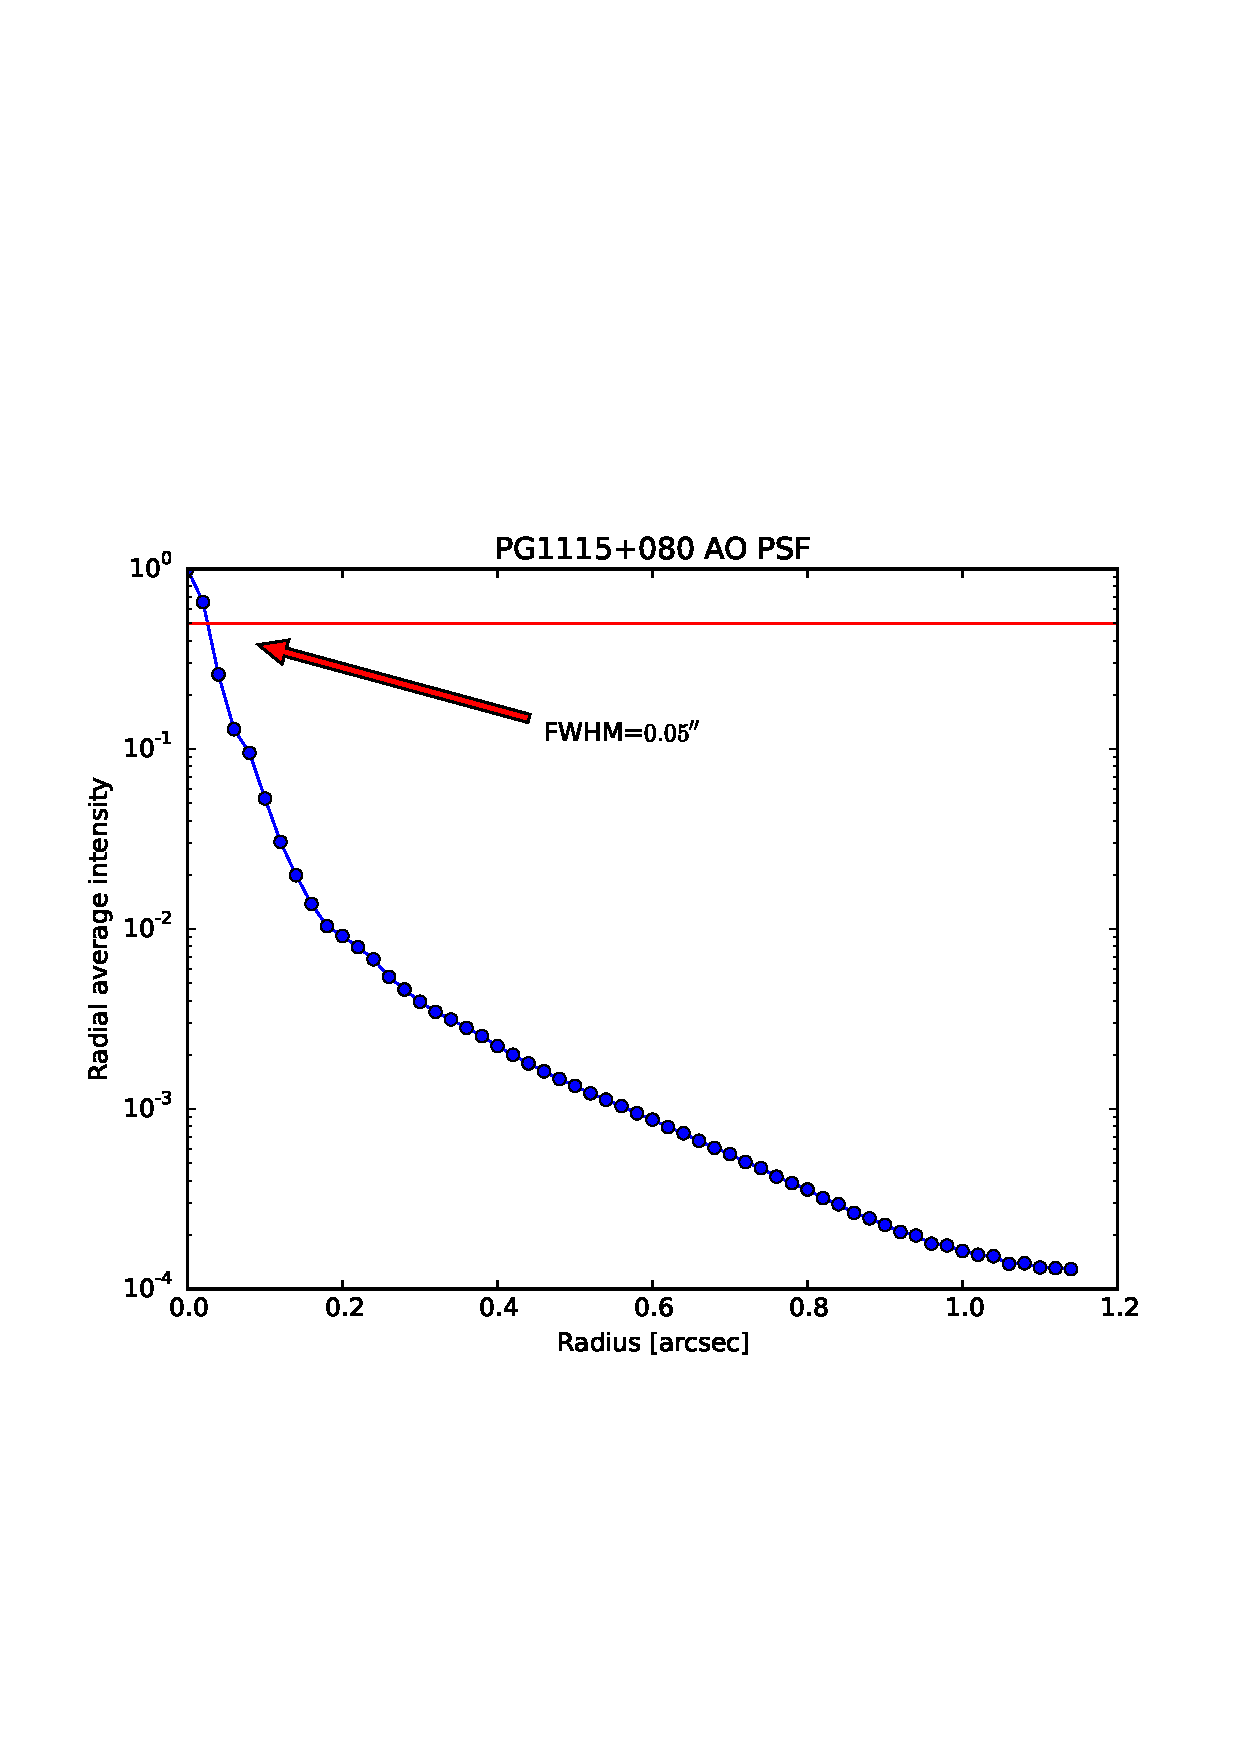
\includegraphics[width=0.5\textwidth, clip]{PG1115_AO_PSF_radius.pdf}
  \caption{The left panel is the reconstructed \pg~AO PSF. The right panel is the radial average intensity of the PSF, which shows the core plus its wings.}
\label{fig:PG1115_AO_PSF}
\end{figure*}

%Under the same modeling strategies, we have done tests on modeling the AO image alone, the HST image alone, and the AO+HST image. 
%We show the comparison of the constraints on Fermat potential with above choices in Fig XX. It shows that AO image alone can provide the comparable constraining power as HST data and AO+HST can provide even tighter constraint on Fermat potential. 
%Thus, combining AO image and HST image can significantly reduce the error budget of the lens mass distribution on the lens plane. 


\begin{figure*}
\centering
\includegraphics[scale=0.6]{PG1115_composite.png}
\caption{test}
\label{fig:PG_composite}
\end{figure*}

\begin{figure*}
\centering
\includegraphics[scale=0.6]{PG1115_powerlaw.png}
\caption{}
\label{fig:PG_pl}
\end{figure*}
%By taking the advantage of using AO image and HST image, the uncertainties of lens modeling on the lens plane significantly decrease. The error budget of $H_{0}$ measurement of \pg~is consequently dominated by the time delays because it is a relatively short time-delay lens. 

\begin{figure*}
\centering
\includegraphics[scale=0.6]{HE0435_AO_image.png}
\caption{\he~AO image reconstruction of the most probable model with a source grid of $50 \times 50$ pixels and $69 \times 69$ pixels PSF for convolution of spatially extended images. Top left: \he~AO image. Top middle: predicted lensed image of the background AGN host galaxy. Top right: predicted light of the lensed AGNs and the lens galaxies. Bottom left: predicted image from all components, which is a sum of the top-middle and top-right panels. Bottom middle: image residual, normalized by the estimated 1$\sigma$ uncertainty of each pixel. Bottom right: the reconstructed host galaxy of the AGN in the source plane. \todo{[Edi: The locations you give do not correspond to the positions of the panels.]}}
\label{fig:HE0435_figure}
\end{figure*}

\begin{figure*}
\centering
\includegraphics[scale=1.0]{HE0435_systematics_tests4.png}
\caption{}
\label{fig:HE0435_Ddt}
\end{figure*}

\begin{figure*}
\centering
\includegraphics[scale=0.8]{RXJ1131_Ddt.png}
\caption{}
\label{fig:RXJ1131_Ddt}
\end{figure*}
\subsubsection{LOS Analysis and the External Convergence}
\todo{[Edi's section]}

\subsubsection{Constraining the Mass-Sheet Transformation}
For every lens model, we calculate the predicted velocity dispersion of the power-law model and the composite model inferred from the lens modeling. We perform the importance sampling given the measured velocity dispersion, $\sigma=281\pm25~\kms$ \citep{Tonry98} inside a 1.0-arcsec$^{2}$ aperture with a seeing of $0.8\arcsec$. The additional constraint on $\kappa_{\textrm{ext}}$ allows us to remove the contribution from the environment and correct the $\Ddt$. Since \pg~is embedded in a nearby group, we check the mass contributed from the group at the location of the lens. It only boosts less than 0.01\% of the velocity dispersion. Thus, we ignore it when calculating the Jeans equation. 

\subsubsection{Systematics Tests and the Unblinding Results}
\label{subsubsec:pg_system}
We summerize the systematic tests for the nearby group/galaxies in the following. 
\begin{description}
  \item[$\bullet$] Main lens: SPEMD+2Serisc; group: NFW with assuming WMAP1 $M_{\textrm{vir}}-c_{\textrm{vir}}$ relationship.
  \item[$\bullet$] Main lens: SPEMD+2Serisc; group: NFW with assuming WMAP3 $M_{\textrm{vir}}-c_{\textrm{vir}}$ relationship.
  \item[$\bullet$] Main lens: SPEMD+2Serisc; group: NFW with assuming WMAP5 $M_{\textrm{vir}}-c_{\textrm{vir}}$ relationship.
  \item[$\bullet$] Main lens: SPEMD+2Serisc; group: NFW with assuming WMAP5 $M_{\textrm{vir}}-c_{\textrm{vir}}$ relationship + G1
  \item[$\bullet$] Main lens: SPEMD+2Serisc; group: SIS + G1
  \item[$\bullet$] Main lens: SPEMD+2Serisc; group: NFW with assuming WMAP5 $M_{\textrm{vir}}-c_{\textrm{vir}}$ relationship + G1 + G2
  \item[$\bullet$] Main lens: Composite; group: NFW with assuming WMAP1 $M_{\textrm{vir}}-c_{\textrm{vir}}$ relationship.
  \item[$\bullet$] Main lens: Composite; group: NFW with assuming WMAP3 $M_{\textrm{vir}}-c_{\textrm{vir}}$ relationship.
  \item[$\bullet$] Main lens: Composite; group: NFW with assuming WMAP5 $M_{\textrm{vir}}-c_{\textrm{vir}}$ relationship.
  \item[$\bullet$] Main lens: Composite; group: NFW with assuming WMAP5 $M_{\textrm{vir}}-c_{\textrm{vir}}$ relationship + G1
  \item[$\bullet$] Main lens: Composite; group: SIS + G1
  \item[$\bullet$] Main lens: Composite; group: NFW with assuming WMAP5 $M_{\textrm{vir}}-c_{\textrm{vir}}$ relationship + G1 + G2
\end{description}
%For each model above, we model the mass of the main lens with both the power-law and the composite model and choose five different source resolutions in order to better control the systematics.
For each model above, we choose five different source resolutions in order to better control the systematics. In adiition, when sampling $\Ddt$ with the time-delay measurements from \citet{BonvinEtal18}, we follow \citet{GChenEtal18a} to sample the $\Ddt$ with/without considering the microlensing time-delay effect. The parameters for estimating the star density and accretion disk model can be found in \citet{GChenEtal18a}. 
In sum, we explore 240 systematics in total with all different choices among two kinds of main lens models, various mass models for the group, 5 different resolution of the reconstructed source, and three different priors of the accretion disk sizes (or we ignore the microlensing time-delay effect). (see detail in appendix \ref{appendix:pg_BIC}). 
In \fref{fig:PG_composite} and \fref{fig:PG_pl}, we present the posteriors of the important parameters of HST+AO results for the composite model and the power-law model, respectively and show the full lens parameters of the power-law model of \pg~in table xx. 

\begin{figure}
%\centering
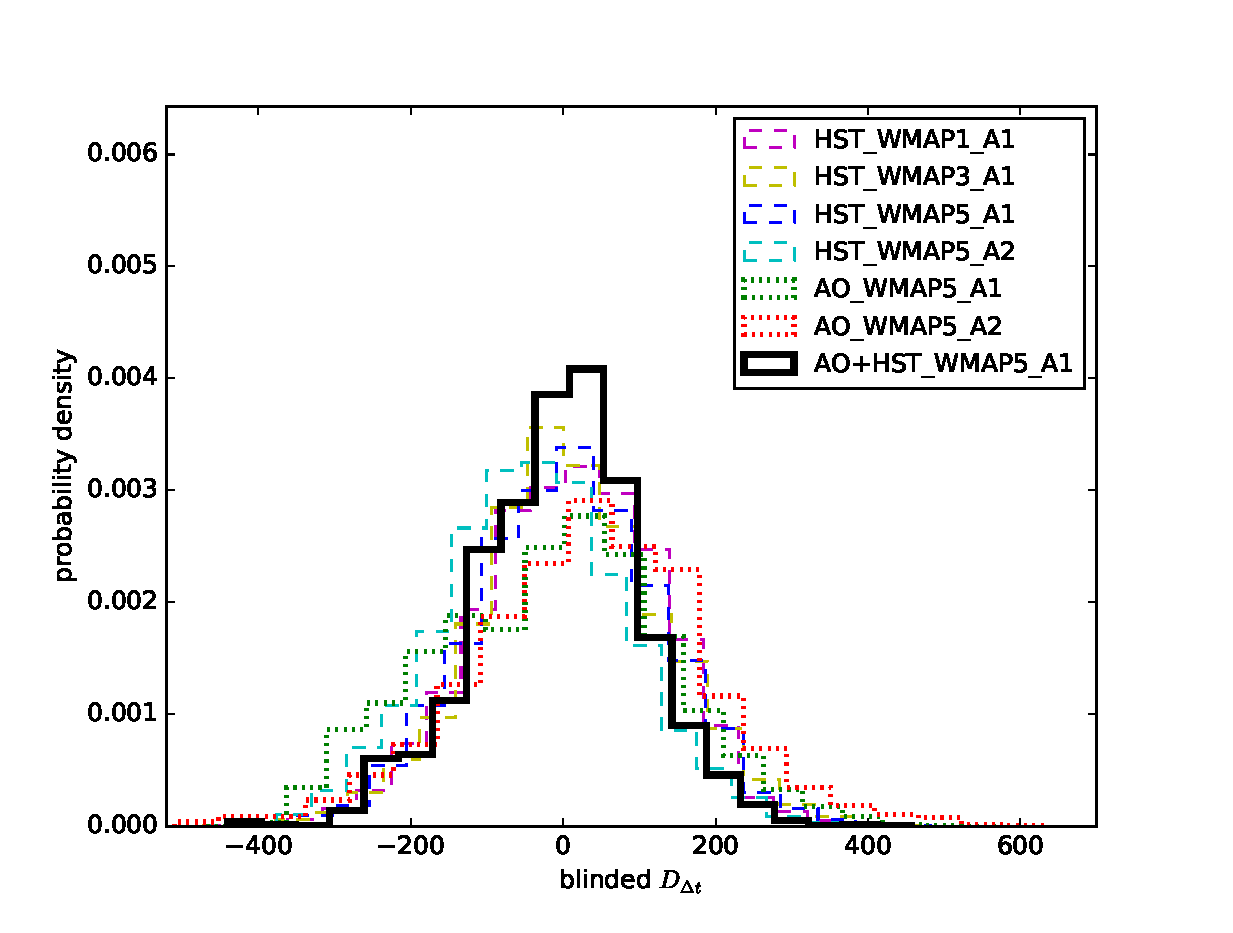
\includegraphics[scale=0.43]{PG1115_systematics_tests.eps}
\caption{}
\label{fig:PG1115_Ddt}
\end{figure}



\subsection{HE0435-1231 modeling}
\label{subsec:HEmodeling}
%Since \he~is a relatively symmetric lens compared with RXJ1131, we expect that the lens will have more degeneracy. In order to make sure that our method also valid in that we are able to recover the important cosmological parameters, a simple mock test is done before applying our method to the real data. (see Appendix \ref{HE0435mocktest}). 
The detailed studies of the environment of \he~can be found in \citet{SluseEtal17}, \citet{RusuEtal17}, and \citet{TihhonovaEtal17}. 
We summarize the important information for performing the lens modeling. 
There are five most important perturbers (G1$\sim$G5) near \he~\citep[see Fig. 3 in][]{WongEtal17}. Based on \citet{McCullyEtal14,McCullyEtal17}, we should include the most massive nearby perturber, G1, explicitly in the model. In addition, \citet{SluseEtal17} show that based on the flexion shifts of the individual perturbers, they are negligible but we should account explicitely for the five nearest perturbers taken together. Since the nearby galaxies are located at different redshift, we follow \citet{WongEtal17} and model this system through multi-plane lens equation \citep[e.g.,][]{BlandfordNarayan86,SEF92,Collett&Auger14,McCullyEtal14,WongEtal17}. In this case, there is no single time-delay distance and a particular cosmological model need to be applied. However, if the lens system is dominated by a main lens such as \he, the time delay is primarily sensitive to the \eref{eq:TDdistance} and insensitive to cosmological models \citep{WongEtal17}. Thus, We can define the effective time-delay distance as $\Ddt^{\textrm{eff}}\left(\zl,\zs\right)$.

\subsubsection{Lens Model choices}
%We briefly describe the modeling strategy and the more detail discussion/arguments can be found in \citet{WongEtal17}.
We model the main lens with either SPEMD or compoiste model. 
%Because G1 is not only a foreground perturber but also close enough to the main lens, its influence cannot simply be described by the external shear \citep{McCullyEtal17}. 
The most massive perturber, G1, is modeled as a SIS profile. Furthermore, We also model the five most significant nearby perturbers rather than just G1 because \citet{SluseEtal17} shows that the five nearest perturbers should be accounted for explicitly based on their flexion shift.
\subsubsection{LOS Analysis and the External Convergence}
\todo{Edi section}

\subsubsection{Constraining the Mass-Sheet Transformation}
For each model, we perform the importance sampling given the measured velocity dispersion, $\sigma=222\pm15~\kms$ \citep{WongEtal17} inside a 0.54-arcsec$^{2}$ aperture with a seeing of $0.8\arcsec$. The additional constraint on $\kappa_{\textrm{ext}}$ allows us to remove the contribution from the environment and correct the $\Ddt$.
\subsubsection{Systematics Tests and Unblinding results}
We list the systematic tests we have done here. Note that we found the $\Ddt$ is stabilized for pixel source larger than $30\times 30$ pixels, so we include the resolution above $30\times 30$ pixels as systematic tests.
\begin{description}
  \item[$\bullet$] A model which includes the most massive nearby galaxy as a SIS and testing different source resolutions $31\times31,~33\times33,~35\times35,~37\times37,~39. \times39$ pixels. We fix the position of the mass center at the center of the light. The regions near the AGN images are given zero weight.
%  \item[$\bullet$] A model includes G1 and the regions near the AGN images are scaled by power-law weighting 
%  \item[$\bullet$] A model includes G1 and the regions near the AGN images given zero weight is increased by one pixel around the outer edge.
%  \item[$\bullet$] A model includes G1 and the regions near the AGN images given zero weight is increased by two pixel around the outer edge.
  \item[$\bullet$] A model which includes the five perturbers. The ratio, assuming SIS, of the Einstein radius are fixed by calculating their stellar mass~\citep{RusuEtal17}. We use ~\citet{BernnardiEtal11} to convert the stellar mass into velocity dispersion.
  \item[$\bullet$] \todo{more?}
\end{description}


\subsubsection{the AO PSF of \he}
For the PSF of AO imaging, we perform 13 times iterative correction and the final PSF has a 95$\times$95 pixel grid ($1.9\arcsec\times1.9\arcsec$). The FWHM of the \he AO PSF is XX and its strehl ratio is XX. We show the reconstructed \he~AO PSF in Fig.~\ref{fig:HE0435_AO_PSF}. 
\begin{figure*}
  \centering
  \includegraphics[width=0.4\textwidth, clip]{HE0435_AO_PSF3.png}
  \includegraphics[width=0.5\textwidth, clip]{HE0435_PSF_radius.png}
  \caption{The left panel is the reconstructed \he~AO PSF. The right panel is the radial average intensity of the PSF, which shows the core plus its wings.}
\label{fig:HE0435_AO_PSF}
\end{figure*}



\subsection{RXJ1131-1231 modeling}
\label{subsec:RXJmodeling}
%\todo{add some background from previous paper}
The detailed discussion about the \rxj~lens modeling can be found in \citet{GChenEtal16}, which we summarize in the following. We use the power-law mass distribution to model the lens potential and use two concentric S$\acute{\text{e}}$rsic profiles to model the lens light. The arc is modeled by the pixelated source grid algorithm and the PSF is directly reconstructed from the four lensed quasar images.
%To overcome the unstable PSF problem, We developed a technique to directly reconstructing the PSF from the AO imaging. 
%The pilot project has demonstrated that AO imaging can provide $50\%$ tighter constraints on $H_{0}$ than \textsl{HST} imaging, in the power-law model \citep{GChenEtal16}. 
%We develop a PSF-reconstructed method to iteratively extract the information directly from the lensed quasar imaging, and by testing the technique with two mock data, we are able to recover the important cosmological parameters. 
To test the systematic uncertainties of the time-delay distance, we also include the composite model with different source resolutions in this paper.
%we also choose different arc masks, different source resolution, and different weighting in the center of AGN.  

\subsubsection{Main Lens}

\subsubsection{LOS Analysis and the External Convergence}

\subsubsection{Constraining the Mass-Sheet Transformation}

\subsubsection{Systematics Tests}
We list the systematic tests we have done here. Note that we have shown the posterior of the $\Ddt$ is stabilized after the source resolution is above $71\times71$ pixels \citep{GChenEtal16}, so we include the different source resolutions above $71\times71$ pixels as systematics tests. We plot the posteriors of $\Ddt$ in Fig \ref{fig:RXJ1131_Ddt}.
\begin{description}
  \item[$\bullet$] A model we have done in \cite{GChenEtal16}, which includes the source resolutions, $71\times71,~73\times73,~75\times75,~77\times77$, and $79\times79$ pixels.  
  The regions near the AGN images are given zero weight. We rerun the model since we did not link the satellite mass position to its light position in \citet{GChenEtal16}. The new results do not show any significant difference.
  \item[$\bullet$] A model which decomposes the baryon and dark matter with constant M/L ratio. 
  The regions near the AGN images are given zero weight.
  The baryon distribution is taken from HST results because the insufficient knowledge of AO PSF wing limits the ability of AO imaging to decompose the baryonic and dark matter due to the degeneracy between reconstructed PSF structure and lens galaxy light. See detailed discussion in \ref{Degeneracy}. We include the models with the different source resolutions, $71\times71,~72\times72,~73\times73,~74\times74$, and $75\times75$ pixels.
%  \item[$\bullet$] A model with 1 pixel with the arcmask region increased by one pixel on both the inner and outer edges. We model it with highest source resolution since it is high enough to compensate for the larger arcmask region
 % \item[$\bullet$] A model where the regions near the AGN images are scaled by power-law weighting
  %\item[$\bullet$] A model where the regions near the AGN images given zero weight is increased by one pixel around the outer edge.
  %\item[$\bullet$] A model where the regions near the AGN images given zero weight is increased by two pixel around the outer edge.
 % \item[$\bullet$] \todo{more?} 
\end{description}


%\section{Joint cosmological analysis}
%\label{sec:jointcosmos}
%Over the past 15 years, with newer and higher precision and accuracy data, the inferred $H_{0}$ and measured $H_{0}$ gradually ends up to different places \citep[see Fig.~1 in][]{Freedman17}. Especially after 2014, an non-negligibly mild tension has raised lots of attention in the cosmology community. Many studies has already tried to resolve this tension assuming the tension is not due to the systematic effect.~\citep{WymanEtal14,HouEtal14,CuestaEtal15,KarwalEtal16,BernalEtal16,ValentinoEtal16,ValentinoEtal17,Romano16,RaczEtal17,EvslinEtal17,SolaEtal17} 
%\todo{add more detail for all the reference list below}
%\citet{WymanEtal14} states that when the number of effective neutrino species is increased in CMB analysis, the expansion rate increases for all times/redshifts, and thus $H_0$ is also a larger value. This alleviates some of the tension between $\planck$ results and supernovae results by shifting the $\planck$ $H_{0}$ distribution into partial agreement with the 68\% c.l. region of \citet{RiessEtal16}. 
%\citet{HouEtal14} investigate the damping tail region through three different partially degenerate extensions of LCDM (helium abundance, effective neutrino species, and the sum of neutrino masses). Larger N$_{\textrm{eff}}$ relieves some tension between CMB, BAO, and H0 measurements of cosmological parameters. Uses WMAP and SPT data sets.
%\citet{CuestaEtal15} discusses calibrating two standard measures: Type Ia supernovae and the BAO. Specifically, this paper discusses the role of the sound horizon in calibrating $H_0$. Figure 2 is useful in seeing the affect of different cosmologies on $H_{0}$. The right panel of Figure 2 shows the sensitivity of the sound horizon to different cosmologies. 
%\citet{BernalEtal16} describe the well-known two promising ways to alter early cosmology, which can alleviate the tension of the current $H_{0}$ tension. These are changing the early time expansion history and changing the details of recombination (see section 4). In section 5, They also describe how to changing late-time cosmology since the CMB is sensitive to both late and early cosmology.
%\citet{Romano16} Romano addressed this question by saying that it is due to the fact that we live in an under-dense region. If we account for the void, the tension can be resolved.
%\citet{RaczEtal17} propose that the nonlinear deviations from a homogeneous FLRW universe (voids and walls) are too great to to account for with perturbation theory. Their numerical simulation models a matter-only CDM universe with a series of what they call “mini-universes,” each with their own local $\Omega_m$ and expansion. They claim that dark energy can be entirely accounted for in this model, as well as the discrepancy between supernova and CMB $H_0$ measurements. 
%\todo{add more detail for all the reference list above}


%Thus, to consolidate the foundation of all the above clever ideas, independent measurements are necessary to test the possible systematics. H0LiCOW team \citep{BonvinEtal17} has already shown that, by using three HST strong lensing imaging, $H_{0}$, in flat $\Lambda$CDM with free matter and energy density, agrees with the local distance ladder measurements of $H_{0}$. To further test and understand the systematic in strong lensing, we show the detail joint cosmological analysis of $H_{0}$ from three AO strong lensing imaging. It is important to emphasize that the results do not completely independent since we use the the same time delays and lens environment of \rxj~and \he~from H0LiCOW team. The main difference is that we use AO imaging and also add a new lens system, \pg, which is not inside the current H0LiCOW samples. The time-delay distance measurement of \rxj~from~\citet{GChenEtal16} was not blind, whereas the measurements of \he~as well as \pg~were done blindly\footnote{The mass profile is not bind when we analyze \he~and \pg.}.

%In \sref{subsec:cosmoAO}, first we check the consistency among $H_{0}$ from the three $\Ddt$ based on the different uniform cosmological models, and then we show the constraint from Time delay Adaptive Optics imaging of three Strong lensing imaging jointly, referred as “TDAOSL” for “Time Delay Adaptive Optics imaging of Strong Lensing.”. In \sref{subsec:beyoundCDM}, we combine TDAOSL with the WMAP Data Release 9 \citep[][hereafter “WMAP”]{BennettEtal13,HinshawEtal13}, and with the $\planck$ 2015 Data Release \citep[][hereafter "$\planck$"]{planck16a}. We also use the combination of $\planck$ data with $\planck$ measurements of CMB weak-lensing \citep[][hereafter "CMBL"]{planck16b}, $\planck$ data with Baryon Acoustic Oscillations surveys at various redshifts \citep[][hereafter BAO]{PercivalEtal10,BeutlerEtal11,BlakeEtal11,AndersonEtal12, PadmanabhanEtal12}, and $\planck$ data with the data of the Joint Light curve Analysis of Supernovae \citep[][hereafter "JLA"]{BetouleEtal13}. We list the cosmological models which we use for the analysis in \tref{table:cosmo_model}. In \sref{subsec:Ddt_compare}, we propose a different point of view on how to use the time delay distance to rank the cosmology models. 



%\begin{table}[ht]
%\caption{Multi-row table}
%\begin{center}
%\begin{tabular}{ccc}
%    \hline
%    \multirow{3}{*}{Multirow}&X\\
%    &X\\&x\\
%    \hline
%\end{tabular}
%\end{center}
%\label{tab:multicol}
%\end{table}



%\begin{table}
%\centering 
%\caption{We list the cosmological models that we test in this work. The first part of the models starting with ``U'' are based on uniform prior of the cosmological parameters, which means that we do not use the information other than TDAOSL. The second part of the model are based on the prior from the WMAP/$\planck$ alone/$\planck$ with CMBL/$\planck$ with CMBL and BAO/$\planck$ with BAO and JLA. See \sref{sec:jointcosmos} for details.}
%\label{table:cosmo_model}
%\begin{tabular}{||c|c||}
%p{3cm}|p{4cm}
%\hline \\[-1em]
% Model name & Description \\ [0.3ex]
% \hline \\[-1em]
% U$H_{0}$ & Flat $\Lambda$CDM cosmology \\
% &$\Omega_{\textrm{m}}=1-\Omega_{\Lambda}=0.32$\\ 
% &$H_{0}$ uniform in [0, 150]   \\  
% &\\
% U$\Lambda$CDM & Flat $\Lambda$CDM cosmology \\
% &$\Omega_{\textrm{m}}=1-\Omega_{\Lambda}$\\
% &$H_{0}$ uniform in [0, 150] \\
% &$\Omega_{\textrm{m}}$ uniform in [0, 1]\\
% &\\
% U$\omega$CDM & Flat $\omega$CDM cosmology \\ 
% &$H_{0}$ uniform in [0, 150] \\
% &$\Omega_{\textrm{de}}$ uniform in [0, 1] \\
% &$\omega$ uniform in [-2.5, 0.5]    \\
% &\\
% Uo$\Lambda$CDM  &Non-flat $\Lambda$CDM cosmology \\
% &$\Omega_{\textrm{k}} =1-\Omega_{\Lambda}-\Omega_{\textrm{m}}$ \\ 
% &$H_{0}$ uniform in [0, 150] \\
% &$\Omega_{\Lambda}$ uniform in [0, 1] \\
% &$\Omega_{\textrm{m}}$ uniform in [0, 1]   \\ [0.3ex]
% \hline \\[-1em]
% o$\Lambda$CDM & Non-flat $\Lambda$CDM cosmology \\
% &WMAP/$\planck$ for $\{H_{0},~\Omega_{\Lambda},~\Omega_{\textrm{m}}\}$\\
% &$\Omega_{\textrm{k}} =1-\Omega_{\Lambda}-\Omega_{\textrm{m}}$\\
% &\\
% N$_{\textrm{eff}}\Lambda$CDM&Flat $\Lambda$CDM\\
% &WMAP/$\planck$ for $\{H_{0},~\Omega_{\Lambda},~N_{\textrm{eff}}\}$\\
% &\\
% m$_{\mu}\Lambda$CDM&Flat $\Lambda$CDM\\
% &WMAP/$\planck$ for $\{H_{0},~\Omega_{\Lambda},~\Sigma\textrm{m}_{\mu}\}$\\
% &\\
% $\omega$CDM&Flat $\omega$CDM\\
% &$\planck$ for $\{H_{0},~\Omega_{\Lambda},~\Omega_{\textrm{de}}\}$\\
% &\\
% N$_{\textrm{eff}}\textrm{m}_{\mu}\Lambda$CDM&Flat $\Lambda$CDM\\
% &$\planck$ for $\{H_{0},~\omega,~\Omega_{\Lambda},~\Sigma \textrm{m}_{\mu},N_{\textrm{eff}}\}$\\
% &\\
% $o\omega$CDM&Open $\Lambda$CDM cosmology\\
% &$\planck$ for $\{H_{0},~\Omega_{\textrm{de}},~\Omega_{\textrm{k}},\omega\}$\\ [0.3ex]
% \hline
% \end{tabular}
%\end{table}


\subsection{Cosmological inference from AO Strong Lensing}
\label{subsec:cosmoAO}
\subsection{Cosmological inference comparison between AO and HST Strong Lensing imaging}
We use the skewed log-normal distribution described in Sec \ref{sec:lens_modeling} to fit the time delay distance distributions of the three lenses and show the parameters used in our joint cosmological analysis in \tref{table:TDfitting}. 

\begin{table}
\centering
\caption{Parameters of the three AO strong lenses used in our analysis. $\mu_{D},~\sigma_{D}$, and $\lambda_{D}$ are related to the analytical fit of the time-delay distance probability function (see...)}
\label{table:TDfitting}
 \begin{tabular}{||c c c c c c||} 
 \hline
 Name & $z_{d}$ & $z_{s}$ & $\mu_{D}$ & $\sigma_{D}$ & $\lambda_{D}$\\ [0.2ex] 
 \hline\hline
 \rxj & 0.295 & 0.658 & 1&1&1 \\ 
 \hline
 \he & 0.4546 & 1.6892 & 1&1&1\\
 \hline
 \pg & 0.31 & 1.722 &  1&1&1\\
 \hline
 
 \end{tabular}

\end{table}

\begin{figure*}
  \centering
  \includegraphics[width=0.28\textwidth,trim=0 0 0 0, clip]{UH0.pdf}
  \includegraphics[width=0.23\textwidth, trim=82 0 0 0,clip]{ULCDM.pdf}
  \includegraphics[width=0.23\textwidth,trim=82 0 0 0,clip]{UwCDM.pdf}
  \includegraphics[width=0.23\textwidth,trim=82 0 0 0, clip]{UoLCDM.pdf}
  \caption{\todo{This is the only the pipeline I use to generate the figures. The value is nothing to do with the current blind AO results.} Marginalized posterior probability distributions for $H_{0}$ in the $UH_{0}$, U$\Lambda$CDM, UwCDM and UoCDM cosmologies using the constraints from the three AO strong lenses (\rxj,~\he,~\pg ). The overlaid histograms present the distributions for each individual strong lens, and the solid black line corresponds to the distribution resulting from the joint inference from all three datasets (TDAOSL). The quoted values of $H_{0}$ in the top-left corner of each panel are the median, 16th and 84th percentiles.}
\label{fig:uniformcosmologies}
\end{figure*}

\subsubsection{Combination of three lenses}
Recall that we introduce an equation in~\sref{subsubsec:comblens} for testing whether two data sets can be combined based on the same cosmological model. If the Bayes factor is larger than 1, it indicates that these two data sets can be combined without loss of any consistency, whereas if the Bayes factor is smaller than one, it indicates that we have some unknown systematic uncertainties, or it might indicate that the true underlying cosmological model is something beyond the current known cosmological models (see the discussion in \sref{subsec:Ddt_compare}).
We use \eref{eq:lognormal} to fit the three probability distribution of three lenses and summarize the results in \tref{table:TDfitting}, and calculate the Bayes factors for the combination of the three lenses based on different cosmological models,
\begin{description}
	\item[$\bullet$] $F_{\textrm{RXJ}\cup\textrm{HE}\cup\textrm{PG}}$ in U$H_{0}$=XX
    \item[$\bullet$] $F_{\textrm{RXJ}\cup\textrm{HE}\cup\textrm{PG}}$ in U$\Lambda$CDM=XX
    \item[$\bullet$] $F_{\textrm{RXJ}\cup\textrm{HE}\cup\textrm{PG}}$ in U$\omega$CDM=XX
    \item[$\bullet$] $F_{\textrm{RXJ}\cup\textrm{HE}\cup\textrm{PG}}$ in Uo$\Lambda$CDM=XX,
\end{description}
and for 1-versus-1 and 2-versus-1 permutations in all cosmological model XXXXXXX.

\subsubsection{Constraints in uniform cosmologies}
Here we present the $H_{0}$ measurement from three AO strong lenses based on different uniform cosmologies in \fref{fig:uniformcosmologies}. We summarize the results.
\begin{description}
	\item[$\bullet$] The $H_{0}=XX\pm XX~\kmsmpc$ with $XX\%$ precision in U$H_{0}$ model
    \item[$\bullet$] The $H_{0}=XX\pm XX~\kmsmpc$ with $XX\%$ precision in U$\Lambda$CDM model
    \item[$\bullet$] The $H_{0}=XX\pm XX~\kmsmpc$ with $XX\%$ precision in U$\omega$CDM model
    \item[$\bullet$] The $H_{0}=XX\pm XX~\kmsmpc$ with $XX\%$ precision in Uo$\Lambda$CDM model
\end{description}

We can see the $H_{0}$ is less constrained in U$\omega$CDM model. The reason is that, as the total energy density is dominated by the dark energy in the late universe, the distance we measured is sensitive to the variation of the normalization of the dark energy density as well as the dark energy equation of state, $\omega$, which leads to the degeneracy between $H_{0}$ and the property of the dark energy.


%\subsection{Comparison between the inferred $\Ddt$ and measured $\Ddt$}
%\label{subsec:Ddt_compare}
%From a different point of view, the true measurements actually are the three $\Ddt$. What if the shift of $H_{0}$ among the three lenses are not from the systematics but from the wrong assumption of the underlying cosmological model? Thus, to fairly compare different models, we want to ask a question that which current cosmological model given the constraint from CMB and BAO gives the best fit to the three $\Ddt$? This method can be extended to the theory which does not require particular parameters (e.g. $H_{0}$)


\section{Conclusions}
\label{sec:conclusion}

\section*{Acknowledgements}
G.~C.-F.~Chen acknowledges support from the Ministry of Education in Taiwan via Government Scholarship to Study Abroad (GSSA).\todo{more?} G.~C.-F.~Chen thank Jen-Wei Hsueh for the useful discussions and feedback. The data presented herein were obtained at the W. M. Keck Observatory, which is operated as a scientific partnership among the California Institute of Technology, the University of California, and the National Aeronautics and Space Administration. The Observatory was made possible by the generous financial support of the W. M. Keck Foundation. The authors wish to recognize and acknowledge the very significant cultural role and reverence that the summit of MaunaKea has always had within the indigenous Hawaiian community. We are most fortunate to have the opportunity to conduct observations from this mountain. This work used computational and storage services associated with the Hoffman2 Shared Cluster provided by UCLA Institute for Digital Research and Education’s Research Technology Group. Data analysis was in part carried out on common use data analysis computer systems at the Astronomy Data Center, ADC, of the National Astronomical Observatory of Japan. 


%%%%%%%%%%%%%%%%%%%%%%%%%%%%%%%%%%%%%%%%%%%%%%%%%%

%%%%%%%%%%%%%%%%%%%% REFERENCES %%%%%%%%%%%%%%%%%%

% The best way to enter references is to use BibTeX:

\bibliographystyle{mnras}
\bibliography{AO_cosmography} % if your bibtex file is called example.bib


% Alternatively you could enter them by hand, like this:
% This method is tedious and prone to error if you have lots of references
%\begin{thebibliography}{99}
%\bibitem[\protect\citeauthoryear{Author}{2012}]{Author2012}
%Author A.~N., 2013, Journal of Improbable Astronomy, 1, 1
%\bibitem[\protect\citeauthoryear{Others}{2013}]{Others2013}
%Others S., 2012, Journal of Interesting Stuff, 17, 198
%\end{thebibliography}

%%%%%%%%%%%%%%%%%%%%%%%%%%%%%%%%%%%%%%%%%%%%%%%%%%

%%%%%%%%%%%%%%%%% APPENDICES %%%%%%%%%%%%%%%%%%%%%

\appendix
%\section{Mock test of HE0435}
%\label{HE0435mocktest}
\section{Degeneracy between AO PSF wing and lens light}
\label{Degeneracy}

%If you want to present additional material which would interrupt the flow of the main paper, it can be placed in an Appendix which appears after the list of references.

\section{Accounting for the missing galaxy group members in PG1115+080 due to spectroscopic incompleteness}
\label{missinggroup_PG1115}

The spectroscopic coverage of the FOV around \pg~is incomplete. Down to $R_c\leq22.5$ and within $120\arcsec$-radius around the lens there are 63 galaxies, out of which 33 have spectroscopy \citep{WilsonEtal16}, 11 of which are part of the galaxy group at $z=0.31$, including the lensing galaxy. This means that there may be other galaxies within this magnitude and radius from the lens which are also part of the galaxy group associated with the lensing galaxy, but which are missed due to spectroscopic incompleteness. In Section~\ref{subsubsect:PG1115group} we have specifically computed the lensing properties of this group, based on its physical properties derived by \citet{WilsonEtal16}. As a result, when we compute $\kappa_\mathrm{ext}$ at the location of the lens, using the weighted number counts approach, we must remove the galaxies which are part of this group, as the convergence from the group has already been included in the lensing models, and must not be double-counted. While the galaxies which are known to be part of the group can easily be removed, we must also account for the galaxies expected to be missed due to our spectroscopic incompleteness. 

We use two different approaches to estimate the number of missing galaxies part of the group. In the first approach we use the knowledge provided by the number of known group members, the number of galaxies with spectroscopy, and the total number of detected galaxies (withing the given magnitude and aperture radius), and we apply Poisson statistics to estimate a number of $10\pm5$ missing galaxies (median and 16th, 84th percentiles). In the second approach we use the group velocity dispersion and virial radius from \citet{WilsonEtal16}, and we estimate the expected number of galaxies inside the virial radius using the empirical relation from \citet{AndreonEtal10}. Using the measured offset from the group centroid to the lens, and propagating all uncertainties, we measure the expected number of missing galaxies at the intersection of the sphere of virial radius and the $120\arcsec$-radius cylinder centered on the lens to be $1^{+3}_{-1}$. We plot the distributions of these numbers in Figure~\ref{fig:missinggroupPG1115}. The first approach predicts a significantly larger number of missing galaxies than the second. In fact, due to the small value of the velocity dispersion, the second method would only predict a total number of $8^{+6}_{-4}$ galaxies, therefore less than the number of confirmed group members, unless we enforce this constraint. As a result, and also due to the fact that it avoids any physical assumption, we consider the first method to be more reliable. A possible shortcoming of our adopted method is that the spectroscopic depth is $R_c\lesssim22.5$, whereas the limiting magnitude to which we applied the weighted number counts approach is $R_c\lesssim23$. However, these two limits are not significantly different, and the small measured velocity dispersion argues against a significantly larger number of group members\protect\footnote{\citet{AndreonEtal10} note that the limiting magnitude they employ corresponds to the Sloan Digital Sky Survey \citep{AdelmanEtal08} completeness at $z\sim0.3$, the redshift of our group. Our deeper data is therefore also complete.}.

\begin{figure}
\includegraphics[width=\linewidth]{estimatinggroupmembersPG1115.png}
\caption{Estimated number of missing galaxy group members inside the $\leq120\arcsec$-radius from the lens system for PG1115+080, computed with two methods, with or without imposing the prior that the group consists of at least the number of galaxies spectroscopically confirmed at the redshift of the group, inside the same aperture.}
\label{fig:missinggroupPG1115}
\end{figure}

\section{Convergence distributions for PG1115+080}
\label{convergence_PG1115}

\begin{figure}
\includegraphics[width=\linewidth]{FOV_PG1115.png}
\caption{$Rc$-band $240\arcsec\times240\arcsec$ image around \pg . This is the same data shown in Figure \ref{fig:PG1115_envir}, but with contrast chosen to better show the detected objects. The large circles mark the $45\arcsec$ and $120\arcsec$ radii apertures centered on the lens. The inner $5\arcsec$ and outer $>120\arcsec$ masked regions are shown in color. For all objects $R\leq23$, small circles mark galaxies and star symbols mark stars.}
\label{fig:fovPG1115}
\end{figure}

\begin{figure*}
\includegraphics[width=\linewidth]{kappahistPG1115Chih-Fan.png}
\caption{Distributions of $\kappa_\mathrm{ext}$ for PG1115+080, for various lens models and their associated shear values. The constraints used to produce the distributions from the MS are the external shear $\gamma$, plus the combination of weighted counts corresponding to galaxy number counts inside the the $45\arcsec$ and $120\arcsec$ apertures, as well as number counts weighted by the inverse of the distance of each galaxy to the lens. In the subscripts of these weights we report the values of the measured median over/underdensities. We used an inner mask of $5\arcsec$ radius around the lens, ignoring the galaxies inside these masks from the weighted counts approach, since these are explicitly incorporated inside the lens models. The size of the histogram bin is $\Delta\kappa_\mathrm{ext}=0.00055$. As the original distributions are noisy, we plot their convolution with a large smoothing window of size $30\times\Delta\kappa_\mathrm{ext}$. The numbers in the lower right side correspond to the medians and standard deviations (the semi-difference of the 84 and 16 percentiles) of the smoothed distributions, in order.}
\label{fig:kappaPG1115}
\end{figure*}

\section{Convergence distributions for HE0435-1223}
\label{convergence_HE0435}
\begin{figure}
\includegraphics[width=\linewidth]{kappahistHE0435Chih-Fan.png}
\caption{Distributions of $\kappa_\mathrm{ext}$ for HE0435-1223, for three different lens models and their associated shear values. The constraints used to produce the distributions from the MS are either the external shear $\gamma$, or the shear plus the combination of weighted counts corresponding to galaxy number counts inside the the $45\arcsec$ aperture, as well as number counts weighted by the inverse of the distance of each galaxy to the lens. For the \texttt{powerlaw + G1} and \texttt{composite + G1} models we used an inner mask of $5\arcsec$ around the lens, and for the \texttt{powerlow + 5 perturbers} model we used a mask of $12\arcsec$ radius\protect\footnote{The five perturbers are indicated in Figure 3 from \citet{WongEtal17}. Three additional galaxies enter the 12\arcsec-radius inner mask, and we slightly boosted their distance from the lens, in order to avoid masking them.}. See the Figure~\ref{fig:kappaHE0435} caption for additional details.}
\label{fig:kappaHE0435}
\end{figure}

\section{Flexion shift of the individual galaxies in PG1115+080}
\label{flexion_shift}
We use Auger et al relations to get the fraction of DM and hence the total mass for the massive galaxies. The other uses relations between stellar mass and velocity dispersion (Zahid et al.). Both of these apply to elliptical galaxies. I get:

\section{Combining the independent measurements}
\label{sec:bayesAOplusHST}
Consider that we have following sets of information, AO imaging ($\bm{d}_{\textrm{AO}}$), HST imaging ($\bm{d}_{\textrm{HST}}$), velocity dispersion ($\sigma$) and environment data ($\bm{d_{\textrm{ENV}}}$), which can be used to constrain the difference of the fermat potential. We already have two independent measurements, $P(\bm{\eta}|\bm{d}_{\textrm{AO}},\textrm{H},\textrm{MS})$ and $P(\bm{\eta}|\bm{d}_{\textrm{HST}}$, $\sigma$, $\bm{d_{\textrm{ENV}}}$,$\textrm{H},\textrm{MS})$, 
 The goal is to combine them and obtain the joint constraint, $P(\bm{\eta}|\bm{d}_{\textrm{HST}},\bm{d}_{\textrm{AO}},\sigma$, $\bm{d_{\textrm{ENV}}},\textrm{H},\textrm{MS})$, where $\bm{\eta}=(\phi_{ij}^{\textrm{H}},\kappa_{\textrm{ext}},\gamma_{\textrm{ext}},\bm{\zeta})$, $\phi_{ij}^{\textrm{H}}$ are the difference of the model fermat potentials (not the true fermat potentail,
$\phi_{ij}^{\textrm{True}}$) at imaging i and j which we are interested, $\kappa_{\textrm{ext}}$ is the convergence from the line of sight, $\gamma_{\textrm{ext}}$ is the external shear inferred from the imaging data, and $\bm{\zeta}$ are the other parameters which we want to marginalize. H is one kind of the lens models (i.g., the power-law model or the composite model) and MS is Millennium Simulation.

We start with the joint constraint and step by step link to the independent measurements. With Bayes’ theorem, the joint constraint can be expressed as
\begin{equation}
\label{bayes}
\begin{split}
P&(\phi_{ij}^{\textrm{H}},\kappa_{\textrm{ext}},\gamma_{\textrm{ext}},\bm{\zeta}|\bm{d}_{\textrm{HST}},\bm{d}_{\textrm{AO}},\sigma, \bm{d_{\textrm{ENV}}},\textrm{H},\textrm{MS})\\
&=P(\bm{d}_{\textrm{HST}},\bm{d}_{\textrm{AO}},\sigma, \bm{d_{\textrm{ENV}}}|\phi_{ij}^{\textrm{H}},\kappa_{\textrm{ext}},\gamma_{\textrm{ext}},\bm{\zeta},\textrm{H},\textrm{MS})\\
&\cdot\frac{P(\phi_{ij}^{\textrm{H}},\kappa_{\textrm{ext}},\gamma_{\textrm{ext}},\bm{\zeta}|\textrm{H},\textrm{MS})}{P(\bm{d}_{\textrm{HST}},\bm{d}_{\textrm{AO}},\sigma, \bm{d_{\textrm{ENV}}}|\textrm{H},\textrm{MS})}, 
\end{split}
\end{equation}
where 
\begin{equation}
\begin{split}
P&(\phi_{ij}^{\textrm{H}},\kappa_{\textrm{ext}},\gamma_{\textrm{ext}},\bm{\zeta}|\textrm{H},\textrm{MS})\\
&=P(\phi_{ij}^{\textrm{H}}|\textrm{H})P(\kappa_{\textrm{ext}}|\textrm{H,MS})P(\gamma_{\textrm{ext}}|\textrm{H})P(\bm{\zeta}|\textrm{H})
\end{split}
\end{equation}
are the priors on the parameters of the mass model and MS. Note that MS naturally provides more $\kappa_{\textrm{ext}}$ which cENVe to mean density and lens model implicitly assumes $\kappa_{\textrm{ext}}<1$, so  $P(\kappa_{\textrm{ext}}|\textrm{H,MS})$ is a non-flat prior with an upper bound ($<1$).


The next step is to separate the datasets into [$\bm{d}_{\textrm{HST}},\sigma, \bm{d_{\textrm{ENV}}}$] and [$\bm{d}_{\textrm{AO}}$]. Since the data are all independent, we can write down
\begin{equation}
\label{eq:separate}
    \begin{split}
        P&(\bm{d}_{\textrm{HST}},\bm{d}_{\textrm{AO}},\sigma, \bm{d_{\textrm{ENV}}}|\phi_{ij}^{\textrm{H}},\kappa_{\textrm{ext}},\gamma_{\textrm{ext}},\bm{\zeta},\textrm{H},\textrm{MS})\\
        &=P(\bm{d}_{\textrm{HST}},\sigma, \bm{d_{\textrm{ENV}}}|\phi_{ij}^{\textrm{H}},\kappa_{\textrm{ext}},\gamma_{\textrm{ext}},\bm{\zeta},\textrm{H},\textrm{MS})\\
        &\cdot P(\bm{d}_{\textrm{AO}}|\phi_{ij}^{\textrm{H}},\kappa_{\textrm{ext}},\gamma_{\textrm{ext}},\bm{\zeta},\textrm{H},\textrm{MS}).
    \end{split}
\end{equation}
Although $\bm{d}_{\textrm{AO}}$ do not have the direct constraint power on $\kappa_{\textrm{ext}}$, the shear value inferred from $\bm{d}_{\textrm{AO}}$ implicitly help constrain $\kappa_{\textrm{ext}}$. Furthermore, we leave $\kappa_{\textrm{ext}}$ in the last term in \eref{eq:separate} because we want to link to $P(\bm{\eta}|\bm{d}_{\textrm{AO}},\textrm{H},\textrm{MS})$ in the future steps. 
\eref{bayes} become
\begin{equation}
\label{inde}
\begin{split}
    &P(\phi_{ij}^{\textrm{H}},\kappa_{\textrm{ext}},\gamma_{\textrm{ext}},\bm{\zeta}|\bm{d}_{\textrm{HST}},\bm{d}_{\textrm{AO}},\sigma, \bm{d_{\textrm{ENV}}},\textrm{H},\textrm{MS})\\
   &=P(\bm{d}_{\textrm{HST}},\sigma, \bm{d_{\textrm{ENV}}}|\phi_{ij}^{\textrm{H}},\kappa_{\textrm{ext}},\gamma_{\textrm{ext}},\bm{\zeta},\textrm{H},\textrm{MS})\\ &\cdot\frac{P(\bm{d}_{\textrm{AO}}|\phi_{ij}^{\textrm{H}},\kappa_{\textrm{ext}},\gamma_{\textrm{ext}},\bm{\zeta},\textrm{H},\textrm{MS})P(\phi_{ij}^{\textrm{H}},\kappa_{\textrm{ext}},\gamma_{\textrm{ext}},\bm{\zeta}|\textrm{H},\textrm{MS})}{P(\bm{d}_{\textrm{HST}},\bm{d}_{\textrm{AO}},\sigma, \bm{d_{\textrm{ENV}}}|\textrm{H},\textrm{MS})},
\end{split}
\end{equation}
where
\begin{equation}
\label{eqe}
\begin{split}
    P&(\bm{d}_{\textrm{HST}},\sigma, \bm{d_{\textrm{ENV}}}|\phi_{ij}^{\textrm{H}},\kappa_{\textrm{ext}},\gamma_{\textrm{ext}},\bm{\zeta},\textrm{H},\textrm{MS})\\
    &=P(\bm{d}_{\textrm{HST}}|\phi_{ij}^{\textrm{H}},\gamma_{\textrm{ext}},\bm{\zeta},\textrm{H})P(\sigma|\phi_{ij}^{\textrm{H}},\kappa_{\textrm{ext}},\gamma_{\textrm{ext}},\bm{\zeta},\textrm{H},\textrm{MS})\\
    &\cdot P(\bm{d_{\textrm{ENV}}}|\gamma_{\textrm{ext}},\kappa_{\textrm{ext}},\textrm{MS}).
\end{split}
\end{equation}
The last term in \eref{eqe} tell us that the shear value inferred from the lens imaging can also help us to further constrain the convergence because of the correlation between the $\gamma_{\textrm{ext}}$and $\kappa_{\textrm{ext}}$ in MS.

Baye's theorem tells us that 
\begin{equation}
\label{eqqee}
\begin{split}
P&(\bm{d}_{\textrm{HST}},\sigma, \bm{d_{\textrm{ENV}}}|\phi_{ij}^{\textrm{H}},\kappa_{\textrm{ext}},\gamma_{\textrm{ext}},\bm{\zeta},\textrm{H},\textrm{MS})\\
&=P(\phi_{ij}^{\textrm{H}},\kappa_{\textrm{ext}},\gamma_{\textrm{ext}},\bm{\zeta}|\bm{d}_{\textrm{HST}},\sigma,\bm{d_{\textrm{ENV}}},\textrm{H},\textrm{MS})\\
&\cdot\frac{P(\bm{d}_{\textrm{HST}},\sigma,\bm{d_{\textrm{ENV}}}|\textrm{H},\textrm{MS})}{P(\phi_{ij}^{\textrm{H}},\kappa_{\textrm{ext}},\gamma_{\textrm{ext}},\bm{\zeta}|\textrm{H},\textrm{MS})},
\end{split}
\end{equation}
and
\begin{equation}
\label{eqqe}
    \begin{split}
        P&(\bm{d}_{\textrm{AO}}|\phi_{ij}^{\textrm{H}},\kappa_{\textrm{ext}},\gamma_{\textrm{ext}},\bm{\zeta},\textrm{H},\textrm{MS})\\
        &=\frac{P(\phi_{ij}^{\textrm{H}},\kappa_{\textrm{ext}},\gamma_{\textrm{ext}},\bm{\zeta}|\bm{d}_{\textrm{AO}},\textrm{H},\textrm{MS})P(\bm{d}_{\textrm{AO}}|\textrm{H},\textrm{MS})}{P(\phi_{ij}^{\textrm{H}},\kappa_{\textrm{ext}},\gamma_{\textrm{ext}},\bm{\zeta}|\textrm{H},\textrm{MS})}.
    \end{split}
\end{equation}
By substituting \eref{eqqee} and \eref{eqqe} into \eref{inde}, finally we obtain
\begin{equation}
\label{final}
\begin{split}
P&(\phi_{ij}^{\textrm{H}},\kappa_{\textrm{ext}},\gamma_{\textrm{ext}},\bm{\zeta}|\bm{d}_{\textrm{HST}},\bm{d}_{\textrm{AO}},\sigma, \bm{d_{\textrm{ENV}}},\textrm{H},\textrm{MS})\\
&\propto P(\phi_{ij}^{\textrm{H}},\kappa_{\textrm{ext}},\gamma_{\textrm{ext}},\bm{\zeta}|\bm{d}_{\textrm{HST}},\sigma, \bm{d_{\textrm{ENV}}},\textrm{H},\textrm{MS})\\
&\cdot\frac{P(\phi_{ij}^{\textrm{H}},\kappa_{\textrm{ext}},\gamma_{\textrm{ext}},\bm{\zeta}|\bm{d}_{\textrm{AO}},\textrm{H},\textrm{MS})}{P(\phi_{ij}^{\textrm{H}},\kappa_{\textrm{ext}},\gamma_{\textrm{ext}},\bm{\zeta}|\textrm{H},\textrm{MS})}.
\end{split}
\end{equation}
%\begin{equation}
%Norm=\frac{P(\bm{d}_{\textrm{HST}},\sigma, \bm{d_{\textrm{ENV}}}|\textrm{H},\textrm{MS})P(\bm{d}_{\textrm{AO}}|\textrm{H},\textrm{MS})}{P(\bm{d}_{\textrm{HST}},\bm{d}_{\textrm{AO}},\sigma, \bm{d_{\textrm{ENV}}}|\textrm{H},\textrm{MS})}.
%\end{equation}
%$Norm$ is not interesting since we have already measured the data. We can treat it like a normalization. 
The first term in the right hand side in \eref{final} is done by \citet{WongEtal17}, while the numerator in the second term is from AO data alone. Thus, based on \eref{final}, in order to get the joint constraint, we need to multiply this two posteriors and divide it by the non-uniform priors (e.g., $P(\kappa_{\textrm{ext}}|\textrm{H,MS})$) used in both datasets. This is because we need to get rid of the extra constraining power from doubly using the same non-uniform priors.
Therefore, the denominator in \eref{final} become $P(\kappa_{\textrm{ext}}|\textrm{H,MS})$.
Note that $\phi_{ij}^{\textrm{H}}$ is the model fermat potential, but what we want to obtain is $P(\phi_{ij}^{\textrm{True}})$, which can be expressed as

\begin{equation}
\begin{split}
P&(\phi_{ij}^{\textrm{True}}|\bm{d}_{\textrm{HST}},\bm{d}_{\textrm{AO}},\sigma, \bm{d_{\textrm{ENV}}},\textrm{H},\textrm{MS})\\
    &=\int d\kappa_{\textrm{ext}}\int d\phi^{\textrm{H}}_{ij}P(\phi^{\textrm{H}}_{ij},\kappa_{\textrm{ext}})\delta(\phi^{\textrm{True}}_{ij}-\phi^{H}_{ij}(1-\kappa_{\textrm{ext}}))\\
    &=\int d\kappa_{\textrm{ext}}\int d\phi^{\textrm{H}}_{ij}P(\phi^{\textrm{H}}_{ij},\kappa_{\textrm{ext}})\frac{\delta(\phi^{\textrm{H}}_{ij}-\phi^{\textrm{True}}_{ij}/(1-\kappa_{\textrm{ext}}))}{|-(1-\kappa_{\textrm{ext}})|}\\
    &=\int d\kappa_{\textrm{ext}}\frac{P(\phi^{\textrm{True}}_{ij}/(1-\kappa_{\textrm{ext}}),\kappa_{\textrm{ext}})}{1-\kappa_{\textrm{ext}}}
\end{split}
\end{equation}
where 
\begin{equation}
\begin{split}
P&(\phi^{\textrm{H}}_{ij},\kappa_{\textrm{ext}})\\
&=\int P(\phi_{ij}^{\textrm{H}},\kappa_{\textrm{ext}},\gamma_{\textrm{ext}},\bm{\zeta}|\bm{d}_{\textrm{HST}},\bm{d}_{\textrm{AO}},\sigma, \bm{d_{\textrm{ENV}}},\textrm{H},\textrm{MS}) d\bm{\zeta} d\gamma_{\textrm{ext}}.
\end{split}
\end{equation}
\section{SUMMARY OF PG1115+080 LENS MODELS WITH RESPECT OF THE BIC VALUE}
\label{appendix:pg_BIC}

%\begin{table*}
%    \centering
%    \caption{All PG1115+080 models ordered in increased BIC value.}
%    \label{tab:6TD}
%    \begin{tabular}{llcccrr}
%        \hline
%        Main lens model & perturbers &$M_{\textrm{vir}}-c_{\textrm{vir}}$& source resolutions & BIC & $\Delta$ BIC & posterior weight\\
%        \hline
%        SPEMD     & group (NFW)+G1+G2 &WMAP5 & $41\times41$ & 16948 & 0  & 1\\ 
%        SPEMD     & group (NFW)+G1+G2 &WMAP5 & $39\times39$ & 16963 & 15 & 0.9967\\ 
%        SPEMD     & group (NFW)+G1    &WMAP5 & $43\times43$ & 16969 & 21 & 0.9869\\ 
%        SPEMD     & group (NFW)       &WMAP3 & $37\times37$ & 16986 & 38 & 0.9707\\ 
%        SPEMD     & group (NFW)+G1    &WMAP5 & $41\times41$ & 16988 & 40 & 0.9485\\ 
%        COMPOSITE & group (NFW)       &WMAP3 & $32\times32$ & 16993 & 45 & 0.9207\\
%        SPEMD     & group (NFW)+G1+G2 &WMAP5 & $37\times37$ & 17015 & 67 & 0.8879\\
%        SPEMD     & group (SIS)~~~+G1    &   & $40\times40$ & 17036 & 88 & 0.8505\\
%        SPEMD     & group (NFW)+G1    &WMAP5 & $39\times39$ & 17051 & 103 & 0.8094\\
%        SPEMD     & group (NFW)       &WMAP5 & $37\times37$ & 17072 & 124 & 0.7652\\
%        SPEMD     & group (NFW)+G1    &WMAP5 & $37\times37$ & 17072 & 124 & 0.7186\\
%        SPEMD     & group (SIS)~~~+G1    &   & $36\times36$ & 17074 & 126 & 0.6704\\
%        SPEMD     & group (NFW)+G1+G2 &WMAP5 & $35\times35$ & 17082 & 134 & 0.6214\\
%        COMPOSITE & group (NFW)+G1    &WMAP5 & $39\times39$ & 17084 & 136 & 0.5721\\
%        COMPOSITE & group (SIS)~~~+G1    &   & $39\times39$ & 17087 & 139 & 0.5232\\
%        SPEMD     & group (NFW)+G1    &WMAP5 & $35\times35$ & 17088 & 140 & 0.4754\\
%        SPEMD     & group (NFW)       &WMAP1 & $38\times38$ & 17095 & 147 & 0.4291\\
%        SPEMD     & group (SIS)~~~+G1 &      & $38\times38$ & 17098 & 150 & 0.3848\\
%        SPEMD     & group (NFW)       &WMAP5 & $38\times38$ & 17100 & 152 & 0.3428\\
%        COMPOSITE & group (NFW)       &WMAP3 & $38\times38$ & 17104 & 156 & 0.3033\\
%        SPEMD     & group (NFW)       &WMAP3 & $36\times36$ & 17111 & 163 & 0.2666\\
%        SPEMD     & group (NFW)       &WMAP3 & $36\times36$ & 17120 & 172 & 0.2328\\
%        COMPOSITE & group (SIS)~~~+G1    &   & $37\times37$ & 17123 & 175 & 0.2020\\
%        SPEMD     & group (SIS)~~~+G1+G2 &   & $33\times33$ & 17128 & 180 & 0.1741\\
%        COMPOSITE & group (NFW)       &WMAP1 & $36\times36$ & 17131 & 183 & 0.1379\\
%        COMPOSITE & group (NFW)       &WMAP5 & $36\times36$ & 17131 & 183 & 0.1379\\
%        SPEMD     & group (SIS)~~~+G1    &   & $34\times34$ & 17137 & 189 & 0.1071\\
%        SPEMD     & group (NFW)       &WMAP1 & $36\times36$ & 17140 & 192 & 0.0899\\
%        COMPOSITE & group (NFW)+G1    &WMAP5 & $35\times35$ & 17141 & 193 & 0.0750\\
%        COMPOSITE & group (NFW)       &WMAP3 & $33\times33$ & 17144 & 196 & 0.0621\\
%        COMPOSITE & group (NFW)       &WMAP1 & $38\times38$ & 17168 & 220 & 0.0511\\
%        COMPOSITE & group (NFW)       &WMAP5 & $38\times38$ & 17169 & 221 & 0.0418\\
%        SPEMD     & group (NFW)       &WMAP3 & $38\times38$ & 17175 & 227 & 0.0339\\
%        SPEMD     & group (NFW)       &WMAP5 & $34\times34$ & 17184 & 236 & 0.0247\\
%        COMPOSITE & group (NFW)       &WMAP3 & $34\times34$ & 17184 & 236 & 0.0247\\
%        COMPOSITE & group (NFW)+G1+G2 &WMAP5 & $37\times37$ & 17187 & 239 & 0.0175\\
%        COMPOSITE & group (SIS)~~~+G1 &      & $35\times35$ & 17194 & 246 & 0.0138\\
%        COMPOSITE & group (NFW)+G1+G2 &WMAP5 & $39\times39$ & 17203 & 255 & 0.0108\\
%        COMPOSITE & group (SIS)~~~+G1 &      & $31\times31$ & 17208 & 260 & 0.0085\\
%        COMPOSITE & group (NFW)+G1+G2 &WMAP5 & $33\times33$ & 17210 & 262 & 0.0066\\
%        COMPOSITE & group (NFW)       &WMAP5 & $32\times32$ & 17214 & 266 & 0.0051\\
%        COMPOSITE & group (NFW)       &WMAP3 & $36\times36$ & 17215 & 267 & 0.0039\\
%        COMPOSITE & group (NFW)+G1    &WMAP5 & $33\times33$ & 17224 & 276 & 0.0029\\
%        COMPOSITE & group (NFW)+G1    &WMAP5 & $37\times37$ & 17231 & 283 & 0.0022\\
%        COMPOSITE & group (NFW)+G1+G2 &WMAP5 & $35\times35$ & 17236 & 288 & 0.0017\\
%        COMPOSITE & group (NFW)       &WMAP5 & $34\times34$ & 17240 & 292 & 0.0012\\
%        SPEMD     & group (NFW)       &WMAP3 & $35\times35$ & 17242 & 294 & 0.0009\\
%        COMPOSITE & group (NFW)       &WMAP1 & $32\times32$ & 17243 & 295 & 0.0007\\
%        SPEMD     & group (NFW)       &WMAP1 & $34\times34$ & 17251 & 303 & 0.0005\\
%        COMPOSITE & group (NFW)+G1+G2 &WMAP5 & $31\times31$ & 17255 & 307 & 0.0004\\
%        SPEMD     & group (NFW)       &WMAP3 & $32\times32$ & 17256 & 308 & 0.0000\\
%        SPEMD     & group (SIS)~~~+G1    &   & $32\times32$ & 17258 & 310 & 0.0000\\
%        COMPOSITE & group (NFW)+G1    &WMAP5 & $32\times32$ & 17231 & 310 & 0.0000\\
%        COMPOSITE & group (NFW)       &WMAP1 & $30\times30$ & 17215 & 311 & 0.0000\\
%        SPEMD     & group (NFW)       &WMAP5 & $32\times32$ & 17260 & 312 & 0.0000\\
%        COMPOSITE & group (SIS)~~~+G1 &      & $33\times33$ & 17261 & 313 & 0.0000\\
%        COMPOSITE & group (NFW)       &WMAP5 & $30\times30$ & 17274 & 326 & 0.0000\\
%        SPEMD     & group (NFW)       &WMAP1 & $30\times30$ & 17291 & 343 & 0.0000\\
%        COMPOSITE & group (NFW)       &WMAP1 & $34\times34$ & 17306 & 358 & 0.0000\\
%        SPEMD     & group (NFW)       &WMAP1 & $33\times33$ & 17344 & 398 & 0.0000\\
%		\hline
%    \end{tabular}
%\end{table*}

\begin{table*}
    \centering
    \caption{Total 240 PG1115+080 models ordered in increased BIC value.}
    \label{tab:6TD_1}
    \begin{tabular}{llccccrr}
        \hline
        Main lens model & perturbers &$M_{\textrm{vir}}-c_{\textrm{vir}}$& accretion disk size & $S_{r}$ & BIC & $\Delta$ BIC & posterior weight\\
        \hline
        SPEMD     & group (NFW)+G1+G2 &WMAP5 & \nomicro   &$41\times41$ & 16955 & 0  & 1\\ 
        COMPOSITE & group (NFW)       &WMAP3 & \nomicro   &$32\times32$ & 16961 & 6 & 0.9968\\
        SPEMD     & group (NFW)+G1    &WMAP5 & \nomicro   &$43\times43$ & 16969 & 14 & 0.9865\\ 
        SPEMD     & group (NFW)+G1+G2 &WMAP5 & \nomicro   &$39\times39$ & 16969 & 14 & 0.9694\\ 
        SPEMD     & group (NFW)       &WMAP3 & \nomicro   &$37\times37$ & 16988 & 33 & 0.9458\\ 
        SPEMD     & group (NFW)+G1    &WMAP5 & \nomicro   &$41\times41$ & 16990 & 35 & 0.9162\\ 
        SPEMD     & group (NFW)+G1+G2 &WMAP5 & $2R_{0}$   &$41\times41$ & 16997 & 42  & 0.8812\\ 
        COMPOSITE & group (NFW)       &WMAP3 & $1R_{0}$   &$32\times32$ & 17003 & 48 & 0.8415\\
        COMPOSITE & group (NFW)       &WMAP3 & $0.5R_{0}$ &$32\times32$ & 17005 & 50 & 0.7978\\
        SPEMD     & group (NFW)+G1+G2 &WMAP5 & $0.5R_{0}$ &$41\times41$ & 17007 & 52  & 0.7511\\ 
        SPEMD     & group (NFW)+G1+G2 &WMAP5 & $1R_{0}$   &$41\times41$ & 17007 & 52  & 0.7020\\
        SPEMD     & group (NFW)+G1+G2 &WMAP5 & \nomicro   &$37\times37$ & 17016 & 61 & 0.6515\\
        COMPOSITE & group (NFW)       &WMAP3 & $2R_{0}$   &$32\times32$ & 17016 & 61 & 0.6003\\
        SPEMD     & group (NFW)+G1    &WMAP5 & $1R_{0}$   &$43\times43$ & 17018 & 63 & 0.5892\\ 
        SPEMD     & group (NFW)+G1+G2 &WMAP5 & $2R_{0}$   &$39\times39$ & 17018 & 63 & 0.4988\\
        SPEMD     & group (NFW)+G1+G2 &WMAP5 & $0.5R_{0}$ &$39\times39$ & 17019 & 64 & 0.4499\\
        SPEMD     & group (NFW)+G1+G2 &WMAP5 & $1R_{0}$   &$39\times39$ & 17019 & 64 & 0.4028\\
        SPEMD     & group (NFW)+G1    &WMAP5 & $0.5R_{0}$ &$43\times43$ & 17022 & 67 & 0.3581\\
        SPEMD     & group (NFW)+G1    &WMAP5 & $2R_{0}$   &$43\times43$ & 17022 & 67 & 0.3161\\
        SPEMD     & group (NFW)       &WMAP3 & $2R_{0}$   &$37\times37$ & 17033 & 78 & 0.2771\\
        SPEMD     & group (NFW)       &WMAP3 & $0.5R_{0}$ &$37\times37$ & 17035 & 80 & 0.2411\\
        SPEMD     & group (NFW)       &WMAP3 & $1R_{0}$   &$37\times37$ & 17036 & 81 & 0.2083\\
        SPEMD     & group (NFW)+G1    &WMAP5 & $0.5R_{0}$ &$41\times41$ & 17039 & 84 & 0.1787\\
        SPEMD     & group (NFW)+G1    &WMAP5 & $2R_{0}$   &$41\times41$ & 17039 & 84 & 0.1522\\
        SPEMD     & group (SIS)~~~+G1 &\nodata& \nomicro   &$40\times40$ & 17041 & 86 & 0.1287\\
        SPEMD     & group (NFW)+G1    &WMAP5 & $1R_{0}$   &$41\times41$ & 17042 & 87 & 0.1081\\
        SPEMD     & group (NFW)+G1    &WMAP5 & \nomicro   &$39\times39$ & 17050 & 95 & 0.0901\\
        COMPOSITE & group (SIS)~~~+G1 &\nodata &\nomicro  &$39\times39$ & 17053 & 98 & 0.0746\\
        COMPOSITE & group (NFW)+G1    &WMAP5 & \nomicro  &$39\times39$ & 17054 & 99 & 0.0613\\
        SPEMD     & group (SIS)~~~+G1 &\nodata& \nomicro  &$36\times36$ & 17069 & 114 & 0.0500\\
        SPEMD     & group (NFW)+G1+G2 &WMAP5 & $0.5R_{0}$&$37\times37$ & 17070 & 115 & 0.0405\\
        SPEMD     & group (NFW)+G1+G2 &WMAP5 & $2R_{0}$  &$37\times37$ & 17070 & 115 & 0.0326\\
        SPEMD     & group (NFW)+G1+G2 &WMAP5 & $1R_{0}$  &$37\times37$ & 17071 & 116 & 0.0260\\
        SPEMD     & group (NFW)+G1    &WMAP5 & \nomicro  &$37\times37$ & 17072 & 117 & 0.0206\\
        SPEMD     & group (NFW)       &WMAP5 & \nomicro  &$37\times37$ & 17074 & 119 & 0.0162\\
        COMPOSITE & group (NFW)       &WMAP3 & \nomicro&$38\times38$ & 17175 & 120 & 0.0127\\
        SPEMD     & group (NFW)+G1    &WMAP5 & \nomicro  &$35\times35$ & 17082 & 127 & 0.0099\\
        SPEMD     & group (NFW)+G1+G2 &WMAP5 & \nomicro  &$35\times35$ & 17083 & 128 & 0.0076\\
        SPEMD     & group (SIS)~~~+G1 &\nodata& $1R_{0}$  &$40\times40$ & 17084 & 129 & 0.0058\\
        SPEMD     & group (SIS)~~~+G1 &\nodata& $2R_{0}$  &$40\times40$ & 17086 & 131 & 0.0044\\
        SPEMD     & group (SIS)~~~+G1 &\nodata& $0.5R_{0}$&$40\times40$ & 17089 & 134 & 0.0033\\
        COMPOSITE & group (NFW)       &WMAP1 & \nomicro&$36\times36$ & 17092 & 137 & 0.0025\\
        COMPOSITE & group (SIS)~~~+G1 &\nodata& \nomicro&$37\times37$ & 17093 & 138 & 0.0019\\
        COMPOSITE & group (NFW)       &WMAP5 & \nomicro&$36\times36$ & 17094 & 139 & 0.0014\\
        SPEMD     & group (SIS)~~~+G1 &\nodata& \nomicro  &$38\times38$ & 17096 & 141 & 0.0010\\
        SPEMD     & group (NFW)       &WMAP1 & \nomicro  &$38\times38$ & 17099 & 144 & 0.0007\\
        SPEMD     & group (NFW)       &WMAP5 & \nomicro  &$38\times38$ & 17099 & 144 & 0.0005\\
        COMPOSITE & group (NFW)+G1 &WMAP5 & $0.5R_{0}$&$39\times39$ & 17099 & 144 & 0.0004\\
        SPEMD     & group (NFW)+G1    &WMAP5 & $1R_{0}$  &$39\times39$ & 17100 & 145 & 0.0000\\
        COMPOSITE & group (NFW)+G1 &WMAP5 & $1R_{0}$&$39\times39$ & 17101 & 146 & 0.0000\\
        COMPOSITE & group (SIS)~~~+G1 &\nodata& $2R_{0}$&$39\times39$ & 17102 & 147 & 0.0000\\
        COMPOSITE & group (NFW)+G1    &WMAP5 & $2R_{0}$&$39\times39$ & 17103 & 148 & 0.0000\\
        SPEMD     & group (NFW)+G1    &WMAP5 & $2R_{0}$  &$39\times39$ & 17104 & 149 & 0.0000\\
        COMPOSITE & group (SIS)~~~+G1 &\nodata& $0.5R_{0}$&$39\times39$ & 17104 & 149 & 0.0000\\
        SPEMD     & group (NFW)+G1    &WMAP5 & $0.5R_{0}$&$39\times39$ & 17106 & 151 & 0.0000\\
        COMPOSITE & group (SIS)~~~+G1 &\nodata& $1R_{0}$&$39\times39$ & 17106 & 151 & 0.0000\\
        COMPOSITE & group (NFW)+G1    &WMAP5 & \nomicro&$35\times35$ & 17107 & 152 & 0.0000\\
        SPEMD     & group (NFW)       &WMAP3 & \nomicro&$36\times36$ & 17110 & 155 & 0.0000\\
        
        \hline
    \end{tabular}
\end{table*}
\begin{table*}
    \centering
    \caption{Total 240 PG1115+080 models ordered in increased BIC value.}
    \label{tab:6TD_2}
    \begin{tabular}{llccccrr}
        \hline
        Main lens model & perturbers &$M_{\textrm{vir}}-c_{\textrm{vir}}$& accretion disk size & $S_{r}$ & BIC & $\Delta$ BIC & posterior weight\\
        \hline
        COMPOSITE & group (NFW)       &WMAP3 & \nomicro&$33\times33$ & 17112 & 157 & 0.0000\\
        SPEMD     & group (NFW)       &WMAP5 & \nomicro&$36\times36$ & 17118 & 163 & 0.0000\\
        COMPOSITE & group (NFW)       &WMAP3 & $1R_{0}$&$38\times38$ & 17118 & 163 & 0.0000\\
        SPEMD     & group (NFW)       &WMAP5 & $2R_{0}$&$37\times37$ & 17119 & 164 & 0.0000\\
        SPEMD     & group (NFW)       &WMAP5 & $1R_{0}$&$37\times37$ & 17120 & 165 & 0.0000\\
        SPEMD     & group (NFW)+G1    &WMAP5 & $2R_{0}$&$37\times37$ & 17120 & 165 & 0.0000\\
        SPEMD     & group (SIS)~~~+G1 &\nodata & $0.5R_{0}$&$36\times36$ & 17121 & 166 & 0.0000\\
        SPEMD     & group (NFW)       &WMAP5 & $0.5R_{0}$&$37\times37$ & 17122 & 167 & 0.0000\\
        SPEMD     & group (SIS)~~~+G1 &\nodata & $2R_{0}$&$36\times36$ & 17122 & 167 & 0.0000\\
        SPEMD     & group (NFW)+G1    &WMAP5 & $1R_{0}$&$37\times37$ & 17122 & 167 & 0.0000\\
        COMPOSITE & group (NFW)       &WMAP3 & $2R_{0}$&$38\times38$ & 17122 & 167 & 0.0000\\
        COMPOSITE & group (NFW)       &WMAP3 & $0.5R_{0}$&$38\times38$ & 17123 & 168 & 0.0000\\
        SPEMD     & group (SIS)~~~+G1 &\nodata& $1R_{0}$&$36\times36$ & 17125 & 170 & 0.0000\\
        SPEMD     & group (NFW)+G1    &WMAP5 & $0.5R_{0}$&$37\times37$ & 17125 & 170 & 0.0000\\
        SPEMD     & group (NFW)+G1+G2 &WMAP5 & \nomicro&$33\times33$ & 17127 & 172 & 0.0000\\
        COMPOSITE & group (NFW)       &WMAP5 & \nomicro&$38\times38$ & 17131 & 176 & 0.0000\\
        SPEMD     & group (NFW)+G1    &WMAP5 & $0.5R_{0}$&$35\times35$ & 17132 & 177 & 0.0000\\
        SPEMD     & group (SIS)~~~+G1 &\nodata& \nomicro&$34\times34$ & 17134 & 179 & 0.0000\\
        SPEMD     & group (NFW)+G1    &WMAP5 & $2R_{0}$&$35\times35$ & 17134 & 179 & 0.0000\\
        COMPOSITE & group (SIS)~~~+G1 &\nodata& $0.5R_{0}$&$37\times37$ & 17135 & 280 & 0.0000\\
        SPEMD     & group (NFW)+G1+G2 &WMAP5 & $0.5R_{0}$&$35\times35$ & 17136 & 181 & 0.0000\\
        SPEMD     & group (NFW)+G1+G2 &WMAP5 & $1R_{0}$&$35\times35$ & 17136 & 181 & 0.0000\\
        COMPOSITE & group (NFW)       &WMAP1 & \nomicro&$38\times38$ & 17137 & 182 & 0.0000\\
        SPEMD     & group (NFW)+G1+G2 &WMAP5 & $2R_{0}$&$35\times35$ & 17140 & 185 & 0.0000\\
        COMPOSITE & group (SIS)~~~+G1 &\nodata& $2R_{0}$&$37\times37$ & 17140 & 185 & 0.0000\\
        SPEMD     & group (NFW)+G1    &WMAP5 & $1R_{0}$&$35\times35$ & 17141 & 186 & 0.0000\\
        SPEMD     & group (NFW)       &WMAP1 & \nomicro&$36\times36$ & 17142 & 187 & 0.0000\\
        SPEMD     & group (NFW)       &WMAP1 & $0.5R_{0}$&$38\times38$ & 17142 & 187 & 0.0000\\
        SPEMD     & group (NFW)       &WMAP1 & $1R_{0}$&$38\times38$ & 17143 & 188 & 0.0000\\
        SPEMD     & group (NFW)       &WMAP1 & $2R_{0}$&$38\times38$ & 17143 & 188 & 0.0000\\
        COMPOSITE & group (NFW)       &WMAP1 & $0.5R_{0}$&$36\times36$ & 17144 & 189 & 0.0000\\
        SPEMD     & group (NFW)       &WMAP5 & $1R_{0}$&$38\times38$ & 17145 & 190 & 0.0000\\
        COMPOSITE & group (SIS)~~~+G1 &\nodata& $1R_{0}$&$37\times37$ & 17145 & 190 & 0.0000\\
        SPEMD     & group (SIS)~~~+G1 &\nodata& $0.5R_{0}$&$38\times38$ & 17146 & 191 & 0.0000\\
        COMPOSITE & group (NFW)       &WMAP1 & $2R_{0}$&$36\times36$ & 17146 & 191 & 0.0000\\
        COMPOSITE & group (NFW)       &WMAP1 & $1R_{0}$&$36\times36$ & 17147 & 192 & 0.0000\\
        COMPOSITE & group (NFW)       &WMAP3 & \nomicro&$34\times34$ & 17147 & 192 & 0.0000\\
        COMPOSITE & group (NFW)       &WMAP5 & $2R_{0}$&$36\times36$ & 17147 & 192 & 0.0000\\
        SPEMD     & group (NFW)       &WMAP5 & $2R_{0}$&$38\times38$ & 17148 & 193 & 0.0000\\
        COMPOSITE & group (NFW)       &WMAP5 & $1R_{0}$&$36\times36$ & 17148 & 193 & 0.0000\\
        SPEMD     & group (NFW)       &WMAP5 & $0.5R_{0}$&$38\times38$ & 17149 & 194 & 0.0000\\
        COMPOSITE & group (NFW)       &WMAP5 & $0.5R_{0}$&$36\times36$ & 17149 & 194 & 0.0000\\
        SPEMD     & group (SIS)~~~+G1 &\nodata& $1R_{0}$&$38\times38$ & 17150 & 195 & 0.0000\\
        SPEMD     & group (SIS)~~~+G1 &\nodata& $2R_{0}$&$38\times38$ & 17152 & 197 & 0.0000\\
        COMPOSITE & group (NFW)+G1    &WMAP5 & $2R_{0}$&$35\times35$ & 17155 & 200 & 0.0000\\
        COMPOSITE & group (NFW)+G1+G2 &WMAP5 & \nomicro&$37\times37$ & 17155 & 200 & 0.0000\\
        SPEMD     & group (NFW)       &WMAP3 & $1R_{0}$&$36\times36$ & 17157 & 202 & 0.0000\\
        COMPOSITE & group (NFW)+G1    &WMAP5 & $1R_{0}$&$35\times35$   & 17157 & 202 & 0.0000\\
        SPEMD     & group (NFW)       &WMAP3 & $2R_{0}$&$36\times36$ & 17158 & 203 & 0.0000\\
        SPEMD     & group (NFW)       &WMAP3 & $0.5R_{0}$&$36\times36$ & 17159 & 204 & 0.0000\\
        COMPOSITE & group (NFW)       &WMAP3 & $2R_{0}$&$33\times33$ & 17161 & 206 & 0.0000\\
        COMPOSITE & group (NFW)+G1    &WMAP3 & $0.5R_{0}$&$35\times35$ & 17161 & 206 & 0.0000\\
        COMPOSITE & group (NFW)       &WMAP3 & $0.5R_{0}$&$33\times33$ & 17162 & 207 & 0.0000\\
        COMPOSITE & group (SIS)~~~+G1 &\nodata& \nomicro&$35\times35$ & 17162 & 207 & 0.0000\\
        COMPOSITE & group (NFW)       &WMAP3 & $1R_{0}$&$33\times33$ & 17163 & 208 & 0.0000\\
        SPEMD     & group (NFW)       &WMAP5 & $1R_{0}$&$36\times36$ & 17166 & 211 & 0.0000\\
        SPEMD     & group (NFW)       &WMAP5 & $0.5R_{0}$&$36\times36$ & 17168 & 213 & 0.0000\\
        SPEMD     & group (NFW)       &WMAP5 & $2R_{0}$&$36\times36$ & 17169 & 214 & 0.0000\\
        SPEMD     & group (NFW)       &WMAP3 & \nomicro&$38\times38$ & 17172 & 217 & 0.0000\\
        COMPOSITE & group (NFW)+G1+G2 &WMAP5 & \nomicro&$39\times39$ & 17172 & 217 & 0.0000\\
        COMPOSITE & group (SIS)~~~+G1 &\nodata& \nomicro&$31\times31$ & 17175 & 220 & 0.0000\\
        
        
        %
        %&&&$\cdots$&&&&\\
        %&&&$\cdots$&&&&\\
        %&&&$\cdots$&&&&\\
        %&&&$\cdots$&&&&\\
        %&&&$\cdots$&&&&\\
        %COMPOSITE & group (NFW)       &WMAP1 & $1R_{0}$&$30\times30$ & 17313 & 363 & 0.0000\\
        %COMPOSITE & group (NFW)       &WMAP1 & $0.5R_{0}$&$30\times30$ & 17316 & 366 & 0.0000\\
        %COMPOSITE & group (NFW)       &WMAP5 & $0.5R_{0}$&$30\times30$ & 17322 & 372 & 0.0000\\
        %COMPOSITE & group (NFW)       &WMAP5 & $1R_{0}$&$30\times30$ & 17326 & 376 & 0.0000\\
        %COMPOSITE & group (NFW)       &WMAP5 & $2R_{0}$&$30\times30$ & 17329 & 379 & 0.0000\\
        %SPEMD     & group (NFW)       &WMAP1 & $1R_{0}$&$30\times30$ & 17339 & 389 & 0.0000\\
        %SPEMD     & group (NFW)       &WMAP1 & $0.5R_{0}$&$30\times30$ & 17340 & 390 & 0.0000\\
        %SPEMD     & group (NFW)       &WMAP1 & $2R_{0}$&$30\times30$ & 17341 & 391 & 0.0000\\
        %SPEMD     & group (NFW)       &WMAP1 & \nomicro&$33\times33$ & 17345 & 395 & 0.0000\\
        %COMPOSITE & group (NFW)       &WMAP1 & $0.5R_{0}$&$34\times34$ & 17350 & 400 & 0.0000\\
        %COMPOSITE & group (NFW)       &WMAP1 & $1R_{0}$&$34\times34$ & 17351 & 401 & 0.0000\\
        %COMPOSITE & group (NFW)       &WMAP1 & $2R_{0}$&$34\times34$ & 17354 & 404 & 0.0000\\
        %SPEMD     & group (NFW)       &WMAP1 & $2R_{0}$&$33\times33$ & 17392 & 402 & 0.0000\\
        %SPEMD     & group (NFW)       &WMAP1 & $0.5R_{0}$&$33\times33$ & 17394 & 444 & 0.0000\\
        %SPEMD     & group (NFW)       &WMAP1 & $1R_{0}$&$33\times33$ & 17396 & 446 & 0.0000\\
        %SPEMD     & group (NFW)       &WMAP5 & &$34\times34$ & 17184 & 236 & 0.0247\\
        %COMPOSITE & group (NFW)       &WMAP3 & &$34\times34$ & 17184 & 236 & 0.0247\\
        %COMPOSITE & group (NFW)+G1+G2 &WMAP5 & &$37\times37$ & 17187 & 239 & 0.0175\\
        %COMPOSITE & group (SIS)~~~+G1 &      & &$35\times35$ & 17194 & 246 & 0.0138\\
        %COMPOSITE & group (NFW)+G1+G2 &WMAP5 & &$39\times39$ & 17203 & 255 & 0.0108\\
        %COMPOSITE & group (SIS)~~~+G1 &      & &$31\times31$ & 17208 & 260 & 0.0085\\
        %COMPOSITE & group (NFW)+G1+G2 &WMAP5 & &$33\times33$ & 17210 & 262 & 0.0066\\
        %COMPOSITE & group (NFW)       &WMAP5 & &$32\times32$ & 17214 & 266 & 0.0051\\
        %COMPOSITE & group (NFW)       &WMAP3 & &$36\times36$ & 17215 & 267 & 0.0039\\
        %COMPOSITE & group (NFW)+G1    &WMAP5 & &$33\times33$ & 17224 & 276 & 0.0029\\
        %COMPOSITE & group (NFW)+G1    &WMAP5 & &$37\times37$ & 17231 & 283 & 0.0022\\
        %COMPOSITE & group (NFW)+G1+G2 &WMAP5 & &$35\times35$ & 17236 & 288 & 0.0017\\
        %COMPOSITE & group (NFW)       &WMAP5 & &$34\times34$ & 17240 & 292 & 0.0012\\
        %SPEMD     & group (NFW)       &WMAP3 & &$35\times35$ & 17242 & 294 & 0.0009\\
        %COMPOSITE & group (NFW)       &WMAP1 & &$32\times32$ & 17243 & 295 & 0.0007\\
        %SPEMD     & group (NFW)       &WMAP1 & &$34\times34$ & 17251 & 303 & 0.0005\\
        %COMPOSITE & group (NFW)+G1+G2 &WMAP5 & &$31\times31$ & 17255 & 307 & 0.0004\\
        %SPEMD     & group (NFW)       &WMAP3 & &$32\times32$ & 17256 & 308 & 0.0000\\
        %SPEMD     & group (SIS)~~~+G1    &   & &$32\times32$ & 17258 & 310 & 0.0000\\
        %COMPOSITE & group (NFW)+G1    &WMAP5 & &$32\times32$ & 17231 & 310 & 0.0000\\
        %COMPOSITE & group (NFW)       &WMAP1 & &$30\times30$ & 17215 & 311 & 0.0000\\
        %SPEMD     & group (NFW)       &WMAP5 & &$32\times32$ & 17260 & 312 & 0.0000\\
        %COMPOSITE & group (SIS)~~~+G1 &      & &$33\times33$ & 17261 & 313 & 0.0000\\
        %COMPOSITE & group (NFW)       &WMAP5 & &$30\times30$ & 17274 & 326 & 0.0000\\
        %SPEMD     & group (NFW)       &WMAP1 & &$30\times30$ & 17291 & 343 & 0.0000\\
        %COMPOSITE & group (NFW)       &WMAP1 & &$34\times34$ & 17306 & 358 & 0.0000\\
        %SPEMD     & group (NFW)       &WMAP1 & &$33\times33$ & 17344 & 398 & 0.0000\\
		\hline
    \end{tabular}
\end{table*}
\begin{table*}
    \centering
    \caption{Total 240 PG1115+080 models ordered in increased BIC value.}
    \label{tab:6TD_3}
    \begin{tabular}{llccccrr}
        \hline
        Main lens model & perturbers &$M_{\textrm{vir}}-c_{\textrm{vir}}$& accretion disk size & $S_{r}$ & BIC & $\Delta$ BIC & posterior weight\\
        \hline
        SPEMD     & group (NFW)+G1+G2 &WMAP5 & $2R_{0}$&$33\times33$ & 17176 & 221 & 0.0000\\
        COMPOSITE & group (NFW)+G1+G2 &WMAP5 & \nomicro&$33\times33$ & 17178 & 223 & 0.0000\\
        SPEMD     & group (NFW)+G1+G2 &WMAP5 & $0.5R_{0}$&$33\times33$ & 17179 & 224 & 0.0000\\
        COMPOSITE & group (NFW)       &WMAP5 & \nomicro&$32\times32$ & 17179 & 224 & 0.0000\\
        SPEMD     & group (NFW)+G1+G2 &WMAP5 & $1R_{0}$&$33\times33$ & 17181 & 226 & 0.0000\\
        COMPOSITE & group (NFW)       &WMAP1 & $1R_{0}$&$38\times38$ & 17182 & 227 & 0.0000\\
        COMPOSITE & group (NFW)       &WMAP3 & \nomicro&$36\times36$ & 17282 & 227 & 0.0000\\
        SPEMD     & group (SIS)~~~+G1 &\nodata& $1R_{0}$&$34\times34$ & 17185 & 230 & 0.0000\\
        COMPOSITE & group (NFW)       &WMAP1 & $0.5R_{0}$&$38\times38$ & 17186 & 231 & 0.0000\\
        COMPOSITE & group (NFW)       &WMAP5 & $1R_{0}$&$38\times38$   & 17186 & 231 & 0.0000\\
        SPEMD     & group (NFW)       &WMAP1 & $0.5R_{0}$&$36\times36$ & 17187 & 232 & 0.0000\\
        SPEMD     & group (SIS)~~~+G1 &\nodata& $0.5R_{0}$&$34\times34$& 17187 & 232 & 0.0000\\
        COMPOSITE & group (NFW)       &WMAP5 & $0.5R_{0}$&$38\times38$ & 17187 & 232 & 0.0000\\
        SPEMD     & group (NFW)       &WMAP5 & \nomicro&$34\times34$   & 17188 & 233 & 0.0000\\
        COMPOSITE & group (NFW)       &WMAP5 & $2R_{0}$&$38\times38$   & 17188 & 233 & 0.0000\\
        COMPOSITE & group (NFW)       &WMAP1 & $2R_{0}$&$38\times38$   & 17189 & 234 & 0.0000\\
        SPEMD     & group (SIS)~~~+G1 &\nodata& $2R_{0}$&$34\times34$  & 17190 & 235 & 0.0000\\
        SPEMD     & group (NFW)       &WMAP1 & $2R_{0}$&$36\times36$   & 17191 & 236 & 0.0000\\
        SPEMD     & group (NFW)       &WMAP1 & $0.5R_{0}$&$36\times36$ & 17192 & 237 & 0.0000\\
        COMPOSITE & group (NFW)+G1    &WMAP5 & \nomicro&$33\times33$   & 17192 & 237 & 0.0000\\
        COMPOSITE & group (NFW)       &WMAP3 & $0.5R_{0}$&$34\times34$ & 17195 & 240 & 0.0000\\
        COMPOSITE & group (NFW)+G1    &WMAP5 & \nomicro&$37\times37$   & 17196 & 241 & 0.0000\\
        COMPOSITE & group (NFW)       &WMAP3 & $1R_{0}$&$34\times34$   & 17200 & 245 & 0.0000\\
        COMPOSITE & group (NFW)+G1+G2 &WMAP5 & $1R_{0}$&$37\times37$   & 17200 & 245 & 0.0000\\
        COMPOSITE & group (NFW)+G1+G2 &WMAP5 & \nomicro&$35\times35$   & 17201 & 246 & 0.0000\\
        COMPOSITE & group (NFW)+G1+G2 &WMAP5 & $0.5R_{0}$&$37\times37$ & 17202 & 247 & 0.0000\\
        COMPOSITE & group (NFW)       &WMAP3 & $2R_{0}$&$34\times34$   & 17203 & 248 & 0.0000\\
        COMPOSITE & group (NFW)+G1+G2 &WMAP5 & $2R_{0}$&$37\times37$   & 17203 & 248 & 0.0000\\
        COMPOSITE & group (NFW)       &WMAP5 & \nomicro&$34\times34$   & 17204 & 249 & 0.0000\\
        COMPOSITE & group (NFW)       &WMAP1 & \nomicro&$32\times32$   & 17210 & 255 & 0.0000\\
        COMPOSITE & group (SIS)~~~+G1 &\nodata   & $2R_{0}$&$35\times35$ & 17211 & 256 & 0.0000\\
        COMPOSITE & group (SIS)~~~+G1 &\nodata   & $1R_{0}$&$35\times35$ & 17213 & 258 & 0.0000\\
        COMPOSITE & group (SIS)~~~+G1 &\nodata   & $0.5R_{0}$&$35\times35$ & 17215 & 260 & 0.0000\\
        COMPOSITE & group (NFW)+G1+G2 &WMAP5 & $2R_{0}$&$39\times39$ & 17216 & 261 & 0.0000\\
        COMPOSITE & group (NFW)+G1+G2 &WMAP5 & $0.5R_{0}$&$39\times39$ & 17219 & 264 & 0.0000\\
        COMPOSITE & group (SIS)~~~+G1 &\nodata & $1R_{0}$&$31\times31$ & 17220 & 265 & 0.0000\\
        COMPOSITE & group (NFW)+G1+G2 &WMAP5 & $1R_{0}$&$33\times33$ & 17221 & 266 & 0.0000\\
        COMPOSITE & group (NFW)+G1+G2 &WMAP5 & $1R_{0}$&$39\times39$ & 17221 & 266 & 0.0000\\
        COMPOSITE & group (SIS)~~~+G1 &\nodata& $0.5R_{0}$&$31\times31$ & 17222 & 267 & 0.0000\\
        COMPOSITE & group (NFW)+G1+G2 &WMAP5 & \nomicro&$31\times31$ & 17222 & 267 & 0.0000\\
        SPEMD     & group (NFW)       &WMAP3 & $2R_{0}$&$38\times38$ & 17223 & 268 & 0.0000\\
        COMPOSITE & group (SIS)~~~+G1 &\nodata   & $2R_{0}$&$31\times31$ & 17224 & 269 & 0.0000\\
        COMPOSITE & group (NFW)+G1    &WMAP5 & \nomicro&$32\times32$ & 17224 & 269 & 0.0000\\
        SPEMD     & group (NFW)       &WMAP3 & $1R_{0}$&$38\times38$ & 17226 & 271 & 0.0000\\
        COMPOSITE & group (NFW)+G1+G2 &WMAP5 & $2R_{0}$&$33\times33$ & 17226 & 271 & 0.0000\\
        COMPOSITE & group (NFW)       &WMAP1 & \nomicro&$30\times30$   & 17227 & 272 & 0.0000\\
        SPEMD     & group (NFW)       &WMAP3 & $0.5R_{0}$&$38\times38$ & 17228 & 273 & 0.0000\\
        COMPOSITE & group (NFW)+G1+G2 &WMAP5 & $0.5R_{0}$&$33\times33$ & 17230 & 275 & 0.0000\\
        SPEMD     & group (NFW)+G1    &WMAP1 & $1R_{0}$&$34\times34$ & 17231 & 276 & 0.0000\\
        COMPOSITE & group (NFW)       &WMAP3 & $0.5R_{0}$&$36\times36$ & 17232 & 277 & 0.0000\\
        COMPOSITE & group (NFW)       &WMAP5 & $2R_{0}$&$32\times32$   & 17232 & 277 & 0.0000\\
        COMPOSITE & group (NFW)       &WMAP3 & $1R_{0}$&$36\times36$   & 17233 & 278 & 0.0000\\
        COMPOSITE & group (NFW)       &WMAP5 & $1R_{0}$&$32\times32$ & 17233 & 278 & 0.0000\\
        COMPOSITE & group (SIS)~~~+G1 &\nodata& \nomicro&$33\times33$   & 17233 & 278 & 0.0000\\
        SPEMD     & group (NFW)       &WMAP5 & $2R_{0}$&$34\times34$ & 17234 & 279 & 0.0000\\
        SPEMD     & group (NFW)       &WMAP5 & $0.5R_{0}$&$34\times34$ & 17235 & 280 & 0.0000\\
        COMPOSITE & group (NFW)       &WMAP3 & $2R_{0}$&$36\times36$ & 17235 & 280 & 0.0000\\
        COMPOSITE & group (NFW)       &WMAP5 & \nomicro&$30\times30$ & 17235 & 280 & 0.0000\\
        COMPOSITE & group (NFW)       &WMAP5 & $0.5R_{0}$&$32\times32$ & 17237 & 282 & 0.0000\\
        COMPOSITE & group (NFW)+G1    &WMAP5 & $2R_{0}$&$33\times33$ & 17239 & 284 & 0.0000\\
        COMPOSITE & group (NFW)+G1    &WMAP5 & $0.5R_{0}$&$33\times33$ & 17240 & 285 & 0.0000\\
        COMPOSITE & group (NFW)+G1    &WMAP5 & $1R_{0}$&$33\times33$ & 17241 & 286 & 0.0000\\
        SPEMD     & group (NFW)       &WMAP3 & \nomicro&$35\times35$ & 17242 & 287 & 0.0000\\
        \hline
    \end{tabular}
\end{table*}

\begin{table*}
    \centering
    \caption{All PG1115+080 models ordered in increased BIC value.}
    \label{tab:6TD_4}
    \begin{tabular}{llccccrr}
        \hline
        Main lens model & perturbers &$M_{\textrm{vir}}-c_{\textrm{vir}}$& accretion disk size & $S_{r}$ & BIC & $\Delta$ BIC & posterior weight\\
        \hline
        COMPOSITE & group (NFW)+G1    &WMAP5 & $0.5R_{0}$&$37\times37$ & 17245 & 290 & 0.0000\\
        COMPOSITE & group (NFW)+G1+G2 &WMAP5 & $1R_{0}$&$35\times35$ & 17247 & 292 & 0.0000\\
        COMPOSITE & group (NFW)+G1    &WMAP5 & $2R_{0}$&$37\times37$ & 17248 & 293 & 0.0000\\
        COMPOSITE & group (NFW)+G1    &WMAP5 & $1R_{0}$&$37\times37$ & 17250 & 295 & 0.0000\\
        COMPOSITE & group (NFW)+G1+G2 &WMAP5 & $2R_{0}$&$35\times35$ & 17251 & 296 & 0.0000\\
        SPEMD     & group (NFW)       &WMAP1 & \nomicro&$34\times34$ & 17252 & 297 & 0.0000\\
        COMPOSITE & group (NFW)+G1+G2 &WMAP5 & $0.5R_{0}$&$35\times35$ & 17256 & 301 & 0.0000\\
        SPEMD     & group (NFW)       &WMAP3 & \nomicro&$32\times32$ & 17257 & 302 & 0.0000\\
        COMPOSITE & group (NFW)       &WMAP5 & $0.5R_{0}$&$34\times34$ & 17257 & 302 & 0.0000\\
        SPEMD     & group (SIS)~~~+G1 &\nodata& \nomicro&$32\times32$ & 17258 & 303 & 0.0000\\
        COMPOSITE & group (NFW)       &WMAP1 & $1R_{0}$&$32\times32$ & 17258 & 303 & 0.0000\\
        COMPOSITE & group (NFW)       &WMAP1 & $2R_{0}$&$32\times32$ & 17258 & 303 & 0.0000\\
        COMPOSITE & group (NFW)       &WMAP5 & $1R_{0}$&$34\times34$ & 17258 & 303 & 0.0000\\
        COMPOSITE & group (NFW)       &WMAP5 & $2R_{0}$&$34\times34$ & 17259 & 304 & 0.0000\\
        SPEMD     & group (NFW)       &WMAP5 & \nomicro&$32\times32$ & 17260 & 305 & 0.0000\\
        COMPOSITE & group (NFW)       &WMAP1 & $0.5R_{0}$&$32\times32$ & 17260 & 305 & 0.0000\\
        COMPOSITE & group (NFW)+G1+G2 &WMAP5 & $1R_{0}$&$31\times31$ & 17270 & 315 & 0.0000\\
        COMPOSITE & group (NFW)+G1+G2 &WMAP5 & $0.5R_{0}$&$31\times31$ & 17271 & 316 & 0.0000\\
        COMPOSITE & group (NFW)+G1+G2 &WMAP5 & $2R_{0}$  &$31\times31$ & 17272 & 317 & 0.0000\\
        COMPOSITE & group (SIS)~~~+G1 &\nodata & $0.5R_{0}$&$33\times33$ & 17273 & 318 & 0.0000\\
        COMPOSITE & group (NFW)+G1    &WMAP5 & $0.5R_{0}$&$32\times32$ & 17273 & 318 & 0.0000\\
        COMPOSITE & group (NFW)+G1    &WMAP5 & $2R_{0}$  &$32\times32$ & 17273 & 318 & 0.0000\\
        COMPOSITE & group (NFW)       &WMAP1 & \nomicro&$34\times34$ & 17274 & 319 & 0.0000\\
        COMPOSITE & group (SIS)~~~+G1 &\nodata&$2R_{0}$ &$33\times33$ & 17274 & 319 & 0.0000\\
        COMPOSITE & group (NFW)+G1    &WMAP5 & $1R_{0}$&$32\times32$ & 17274 & 319 & 0.0000\\
        COMPOSITE & group (NFW)       &WMAP1 & \nomicro&$30\times30$ & 17277 & 322 & 0.0000\\
        COMPOSITE & group (SIS)~~~+G1 &\nodata&$1R_{0}$ &$33\times33$ & 17279 & 324 & 0.0000\\
        COMPOSITE & group (NFW)       &WMAP1 & $1R_{0}$&$30\times30$ & 17280 & 325 & 0.0000\\
        COMPOSITE & group (NFW)       &WMAP1 & $0.5R_{0}$&$30\times30$ & 17283 & 328 & 0.0000\\
        SPEMD     & group (NFW)       &WMAP1 & \nomicro&$30\times30$ & 17285 & 330 & 0.0000\\
        SPEMD     & group (NFW)       &WMAP3 & $0.5R_{0}$&$35\times35$ & 17287 & 332 & 0.0000\\
        COMPOSITE & group (NFW)       &WMAP5 & $0.5R_{0}$&$30\times30$ & 17289 & 334 & 0.0000\\
        SPEMD     & group (NFW)       &WMAP3 & $1R_{0}$&$35\times35$ & 17292 & 337 & 0.0000\\
        SPEMD     & group (NFW)       &WMAP3 & $2R_{0}$&$35\times35$ & 17292 & 337 & 0.0000\\
        COMPOSITE & group (NFW)       &WMAP5 & $1R_{0}$&$30\times30$ & 17293 & 338 & 0.0000\\
        SPEMD     & group (NFW)       &WMAP1 & $1R_{0}$&$34\times34$ & 17296 & 341 & 0.0000\\
        COMPOSITE & group (NFW)       &WMAP5 & $2R_{0}$&$30\times30$ & 17296 & 341 & 0.0000\\
        SPEMD     & group (NFW)       &WMAP1 & $2R_{0}$&$34\times34$ & 17302 & 347 & 0.0000\\
        SPEMD     & group (NFW)       &WMAP3 & $1R_{0}$&$32\times32$ & 17303 & 348 & 0.0000\\
        SPEMD     & group (SIS)~~~+G1 &\nodata& $2R_{0}$&$32\times32$ & 17304 & 349 & 0.0000\\
        SPEMD     & group (NFW)       &WMAP3 & $2R_{0}$&$32\times32$ & 17305 & 350 & 0.0000\\
        SPEMD     & group (NFW)       &WMAP1 & $0.5R_{0}$&$34\times34$ & 17306 & 351 & 0.0000\\
        SPEMD     & group (SIS)~~~+G1 &\nodata& $1R_{0}$&$32\times32$ & 17306 & 351 & 0.0000\\
        SPEMD     & group (NFW)       &WMAP3 & $0.5R_{0}$&$32\times32$ & 17307 & 352 & 0.0000\\
        SPEMD     & group (NFW)       &WMAP5 & $0.5R_{0}$&$32\times32$ & 17307 & 352 & 0.0000\\
        SPEMD     & group (SIS)~~~+G1 &\nodata & $0.5R_{0}$&$32\times32$ & 17307 & 352 & 0.0000\\
        SPEMD     & group (NFW)       &WMAP5 & $1R_{0}$&$32\times32$ & 17309 & 354 & 0.0000\\
        SPEMD     & group (NFW)       &WMAP5 & $2R_{0}$&$32\times32$ & 17312 & 357 & 0.0000\\
        COMPOSITE & group (NFW)       &WMAP1 & $0.5R_{0}$&$34\times34$ & 17317 & 362 & 0.0000\\
        COMPOSITE & group (NFW)       &WMAP1 & $1R_{0}$&$34\times34$ & 17318 & 363 & 0.0000\\
        COMPOSITE & group (NFW)       &WMAP1 & $2R_{0}$&$34\times34$ & 17321 & 366 & 0.0000\\
        SPEMD     & group (NFW)       &WMAP1 & $1R_{0}$&$30\times30$ & 17339 & 384 & 0.0000\\
        SPEMD     & group (NFW)       &WMAP1 & $0.5R_{0}$&$30\times30$ & 17340 & 385 & 0.0000\\
        SPEMD     & group (NFW)       &WMAP1 & $2R_{0}$&$30\times30$ & 17341 & 386 & 0.0000\\
        SPEMD     & group (NFW)       &WMAP1 & \nomicro&$33\times33$ & 17345 & 390 & 0.0000\\
        SPEMD     & group (NFW)       &WMAP1 & $2R_{0}$&$33\times33$ & 17392 & 437 & 0.0000\\
        SPEMD     & group (NFW)       &WMAP1 & $0.5R_{0}$&$33\times33$ & 17394 & 439 & 0.0000\\
        SPEMD     & group (NFW)       &WMAP1 & $1R_{0}$&$33\times33$ & 17396 & 441 & 0.0000\\
        \hline
    \end{tabular}
\end{table*}
%%%%%%%%%%%%%%%%%%%%%%%%%%%%%%%%%%%%%%%%%%%%%%%%%%


% Don't change these lines
\bsp	% typesetting comment
\label{lastpage}
\end{document}

% End of mnras_template.tex